 \mychapter{Geometria a l'espai}{Geometria a l'espai}{\begin{center}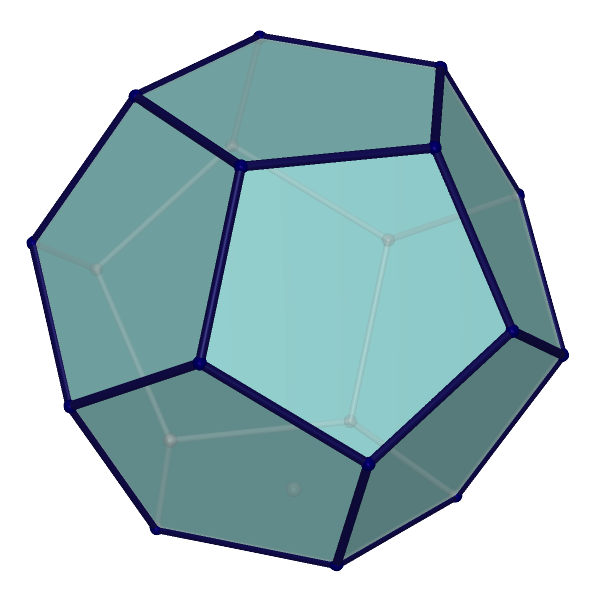
\includegraphics[width=0.9\textwidth]{img-11/dodecaedre} \footnotesize Dodecaedre. Polígon regular de \linebreak 12 cares\end{center}}{chap:geo3d}

\section{Perpendicularitat i paral·lelisme a l'espai}

\begin{mylist}
	
\vspace{-2.5cm}
\exer \begin{minipage}[t]{0.6\textwidth}
Cerca a l'habitació en la qual et trobes, exemples de:
	
	\begin{tasks}
		\task  Plans paral·lels i perpendiculars. 
		
		\task  Rectes paral·leles, rectes perpendiculars i coplanàries, rectes perpendiculars i no coplanàries.
		
		\task  Recta paral·lela al pla, recta i plans secants, recta continguda en pla.
	\end{tasks}

\end{minipage}
\begin{minipage}{0.3\textwidth}
	\centering
	\vspace{2.5cm}
	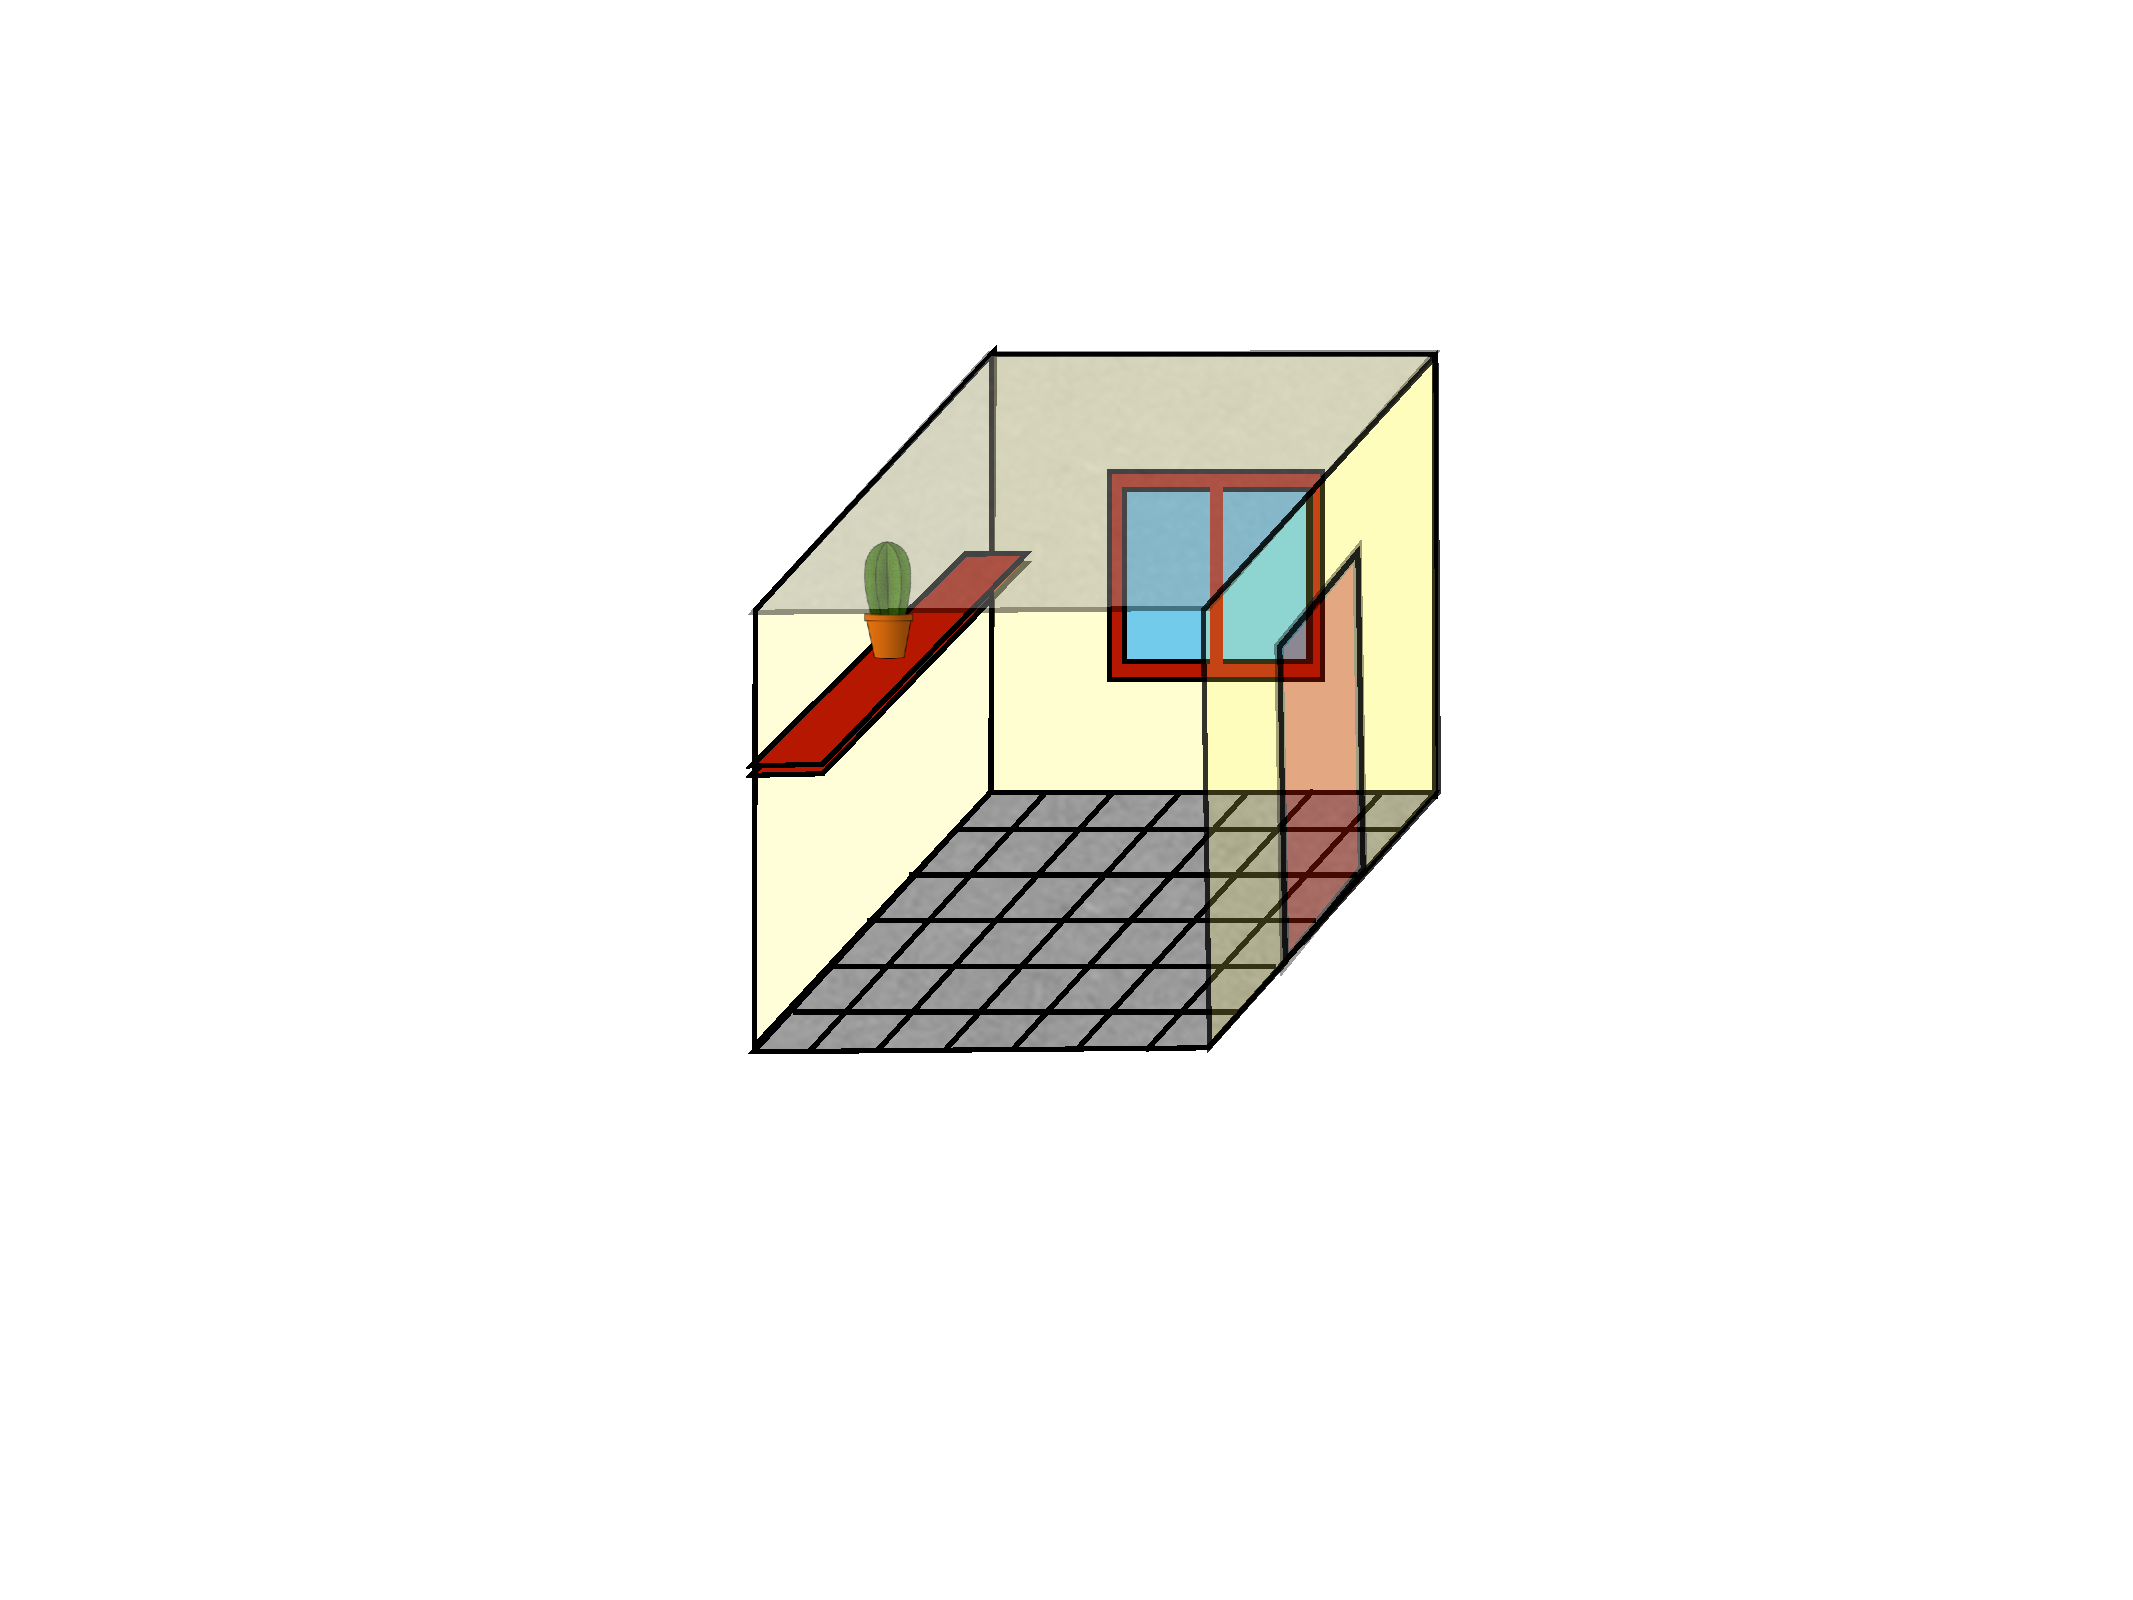
\includegraphics[width=0.97\textwidth]{img-11/habitacio}
\end{minipage}

\answers[cols=1]{[El terra i el sòtil són plans paral·lels. El terra i una paret són plans perpendiculars, El rodapeus de cada banda de classe són rectes paral·leles, etc.]}


\exer  Les fulles d'una porta giratòria formen entre sí 5 angles diedres consecutius i iguals. Quant mesura cadascun d'ells?
\answers{Angle de 72$^\circ$}

\exer  Des d'un punt interior a una sala de planta hexagonal regular es traça una recta perpendicular a cada paret. Quant mesurarà l'angle que formen dues perpendiculars consecutives?
\answers{Angle de 60$^\circ$}

\exer  Dos triedres tenen les tres cares iguals, es pot assegurar que són iguals? Raona la resposta.
\answers{Han d'ésser iguals els tres diedres que el formen.}

\end{mylist}
 
\pagebreak

\section{ Poliedres }

\begin{theorybox}
 Un poliedre és un cos geomètric format per cares planes. Una aresta és allà on s'ajunten dues cares. Un vèrtex és el punt on es troben dues arestes.

 \begin{multicols}{2}
 	 	\centering
 	 \textbf{Poliedre còncau}
 	
 	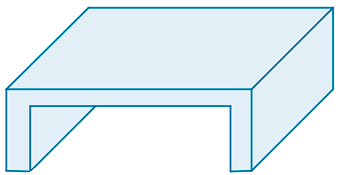
\includegraphics[height=2cm]{img-11/poliedro-concavo}
 	
  {\scriptsize	Algunes de les seves cares no es poden recolçar sobre un pla.}
 	
 	\textbf{Poliedre convex}
 		
 	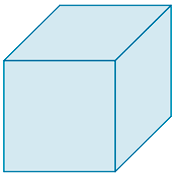
\includegraphics[height=2cm]{img-11/poliedro-convexo}
 	
 	{\scriptsize	Totes les seves cares sí es poden recolçar sobre un pla.}
 \end{multicols}
	
 La \textbf{relació d'Euler} estableix una relació entre el nombre de cares ${C}$, arestes $A$ i vèrtex $V$ que pot tenir un \textbf{políedre convex}:	
 \[C+V=A+2\]
 
\end{theorybox}

\begin{mylist}
\exer \mental Investiga si els següents cossos són poliedres i, en cas afirmatiu, si compleixen el teorema de \textit{Euler}. Indica també si són còncaus o convexos


\begin{longtable}{p{0.9in}p{0.9in}p{0.9in}p{1.0in}p{0.8in}} 
a) 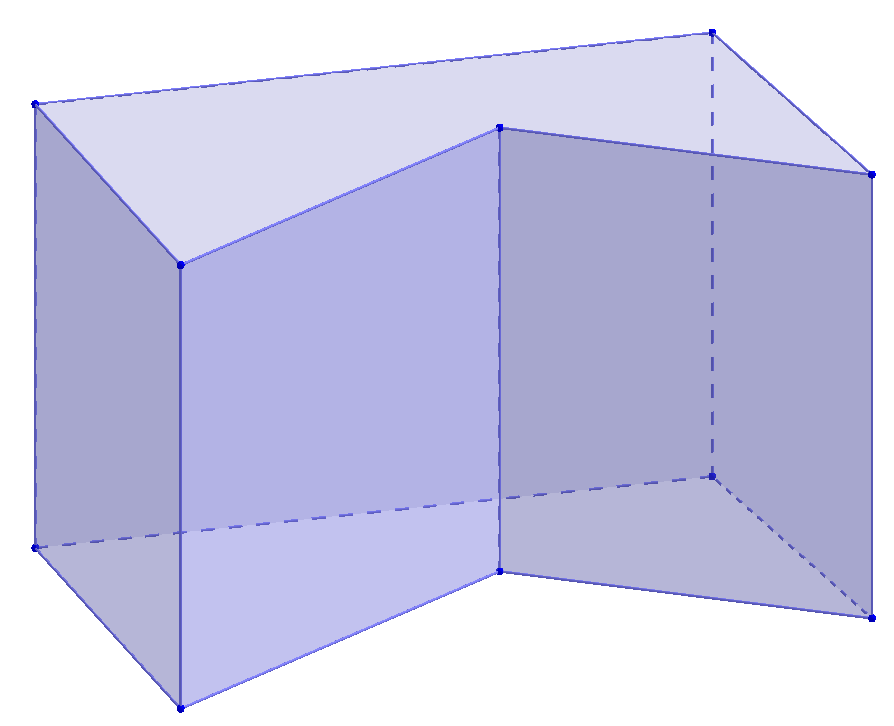
\includegraphics[width=1in]{img-11/prisma1} & 
b) 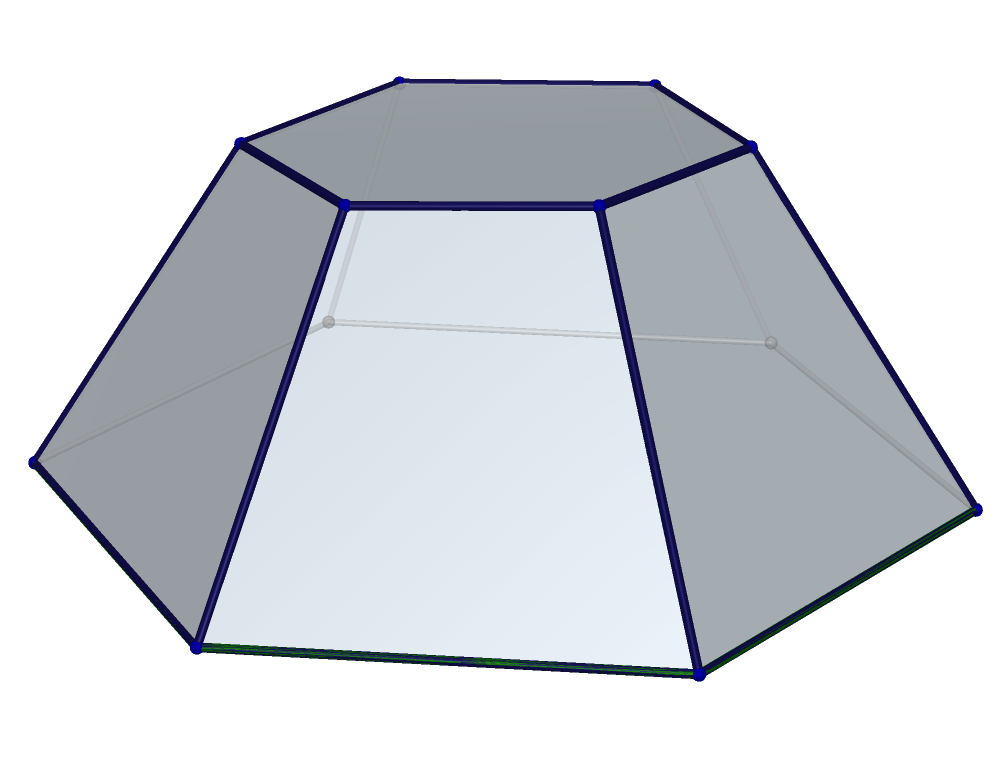
\includegraphics[width=1in]{img-11/tronc11} & 
c) 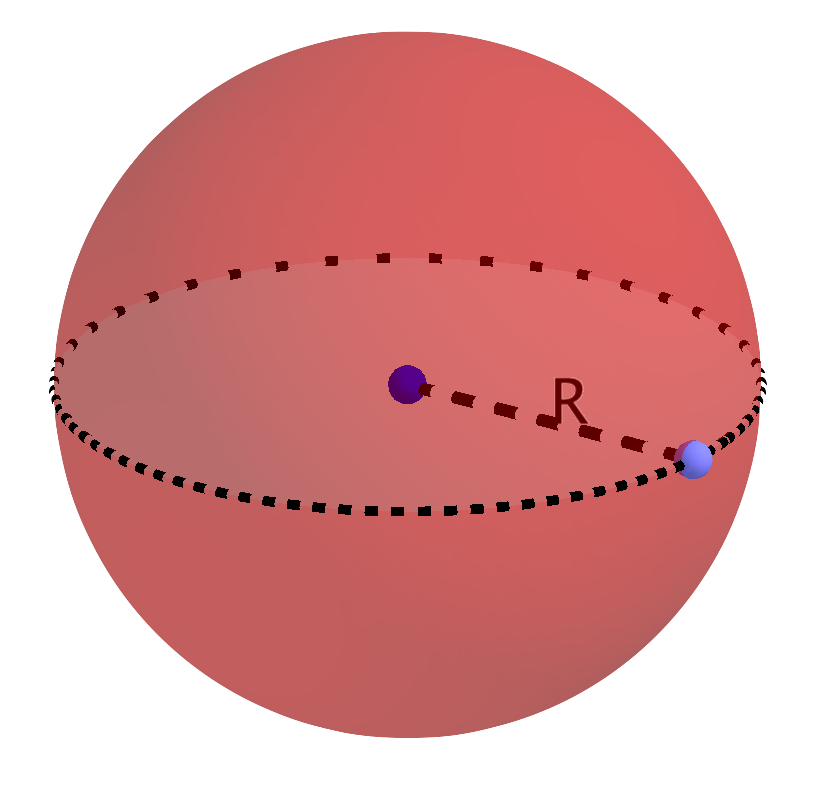
\includegraphics[width=1in]{img-11/esfera} & 
d) 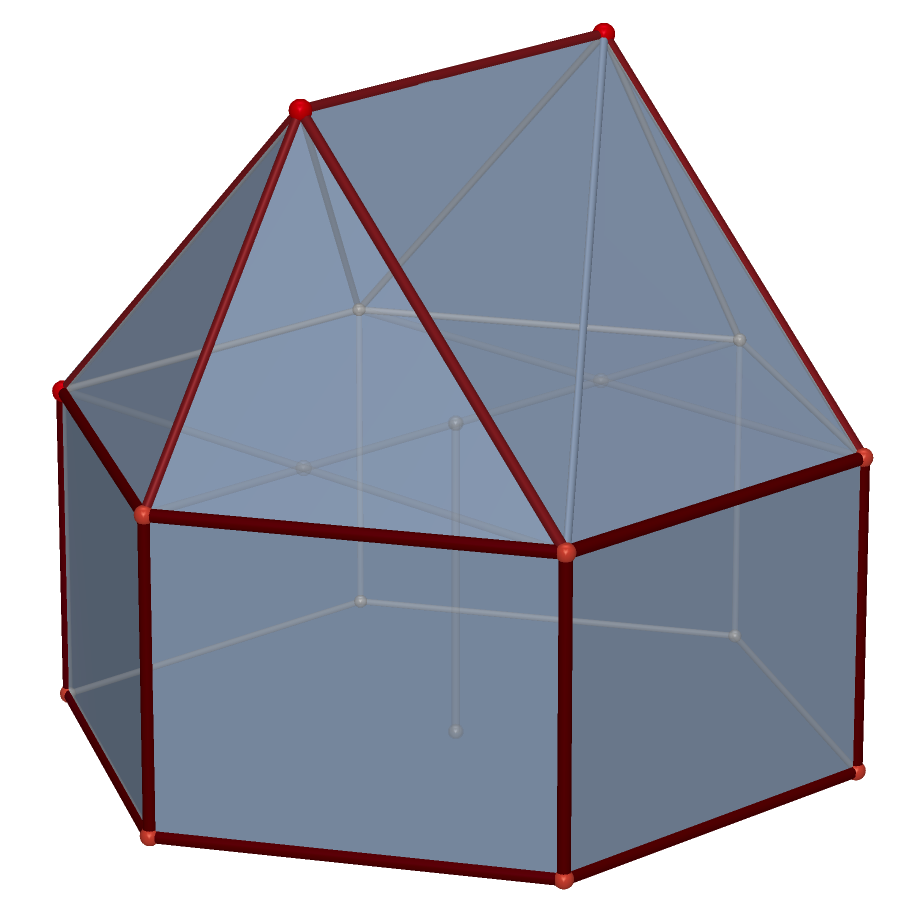
\includegraphics[width=1in]{img-11/raro} & e) 
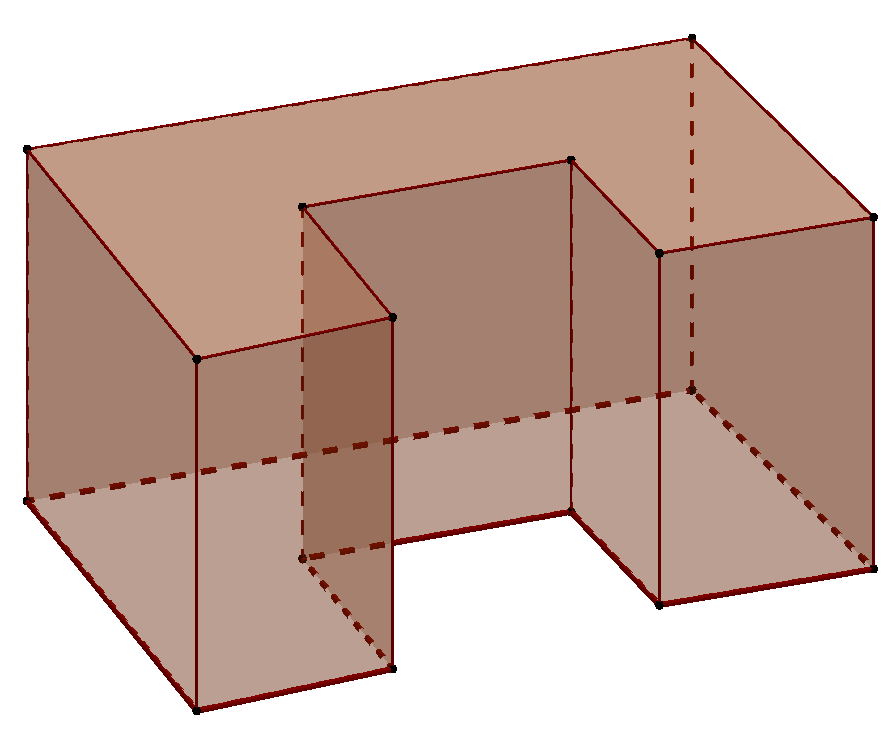
\includegraphics[width=1in]{img-11/prisma2} \\ 

Poliedre?\par Convex?\par C=\par V=\par A=\par Euler? & Poliedre?\par Convex?\par C=\par V=\par A=\par Euler? & Poliedre?\par Convex?\par C=\par V=\par A=\par Euler? & Poliedre?\par Convex?\par C=\par V=\par A=\par Euler? & Poliedre?\par Convex?\par  C=\par V=\par A=\par Euler? \\
\end{longtable}

\answers[cols=1]{[Poliedre. No convex. $C=7$; $V=10$; $A=15$. Euler $7+10 = 15+2$,
	 Poliedre. Convex. $C=8$; $V=12$; $A=18$. Sí Euler $8+12=18+2$,
	 No Poliedre.,
	 Poliedre. Convex. $C=13$; $V=14$; $A=25$. Sí Euler $13+14=25+2$,
	 Poliedre. No convex. $C=10$; $V=16$; $A=24$. Euler $10+16=24+2$]}

\end{mylist}

\begin{theorybox}
	Un políedre és regular si totes les seves cares són igual i si a cada vèrtex hi conflueix el mateix nombre cares i d'arestes.
	
	Només existeixen 5 políedres regulars (sòlids platònics):
	\begin{center}
		\begin{tabular}{|c|c|c|c|c|}\hline
			\rowcolor{lightgray} Tetraedre & Cub & Octaedre & Dodecaedre & Icosaedre \\ \hline
			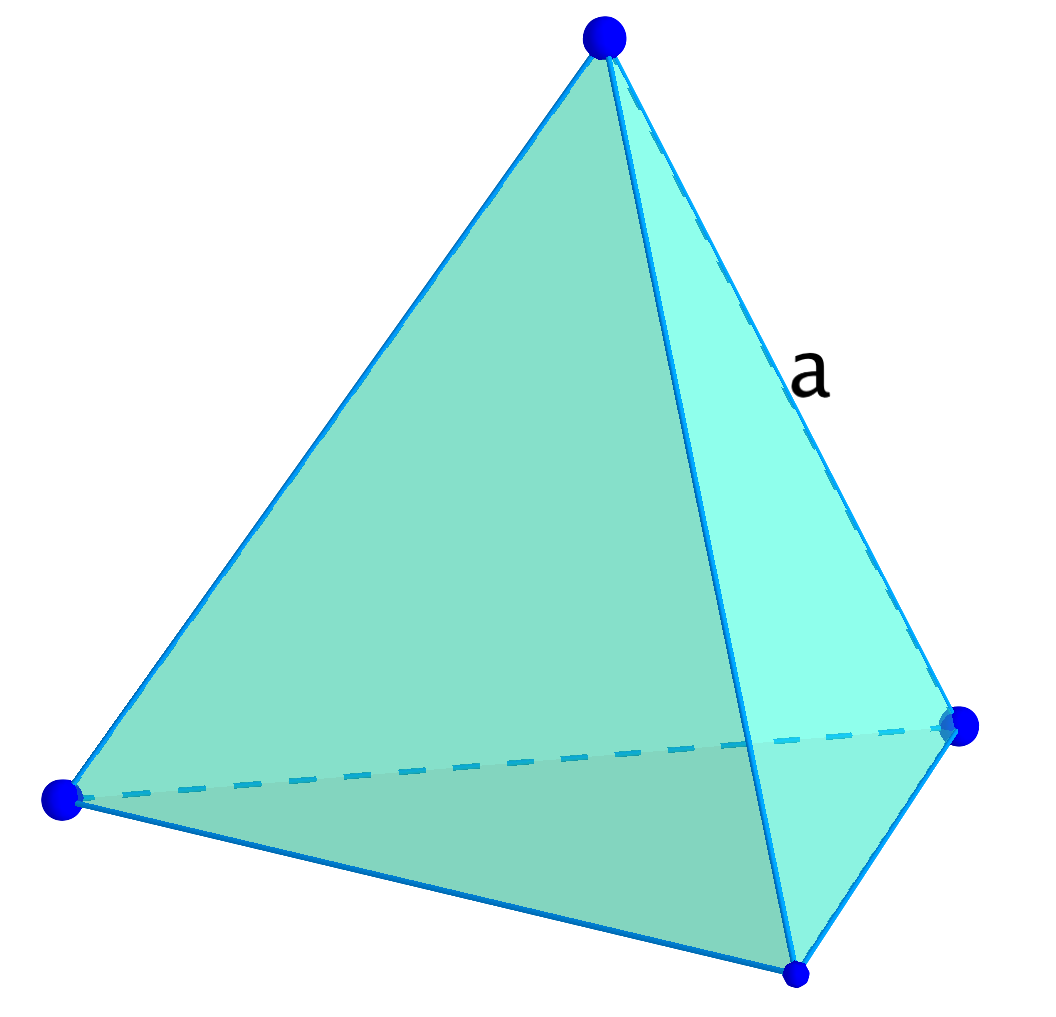
\includegraphics[width=0.15\textwidth]{img-11/tetraedro} &
			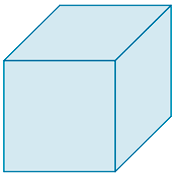
\includegraphics[width=0.15\textwidth]{img-11/poliedro-convexo} &
			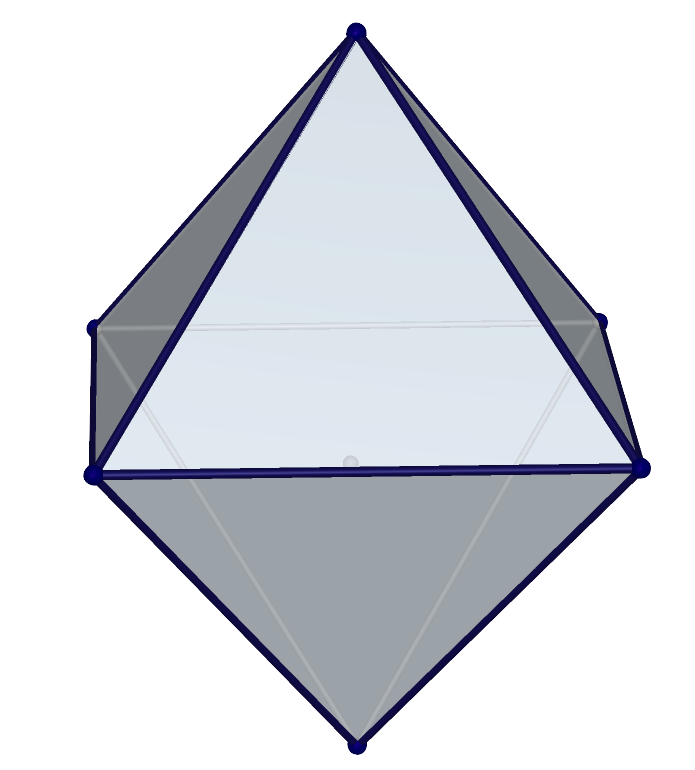
\includegraphics[width=0.15\textwidth]{img-11/octaedre} &
			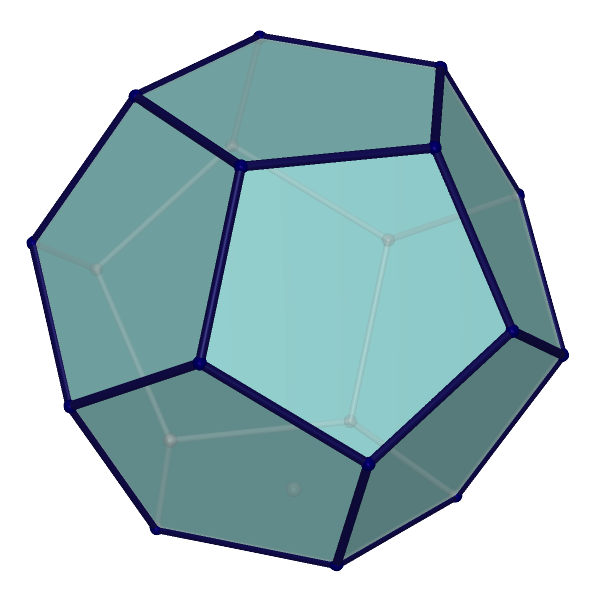
\includegraphics[width=0.15\textwidth]{img-11/dodecaedre} &
			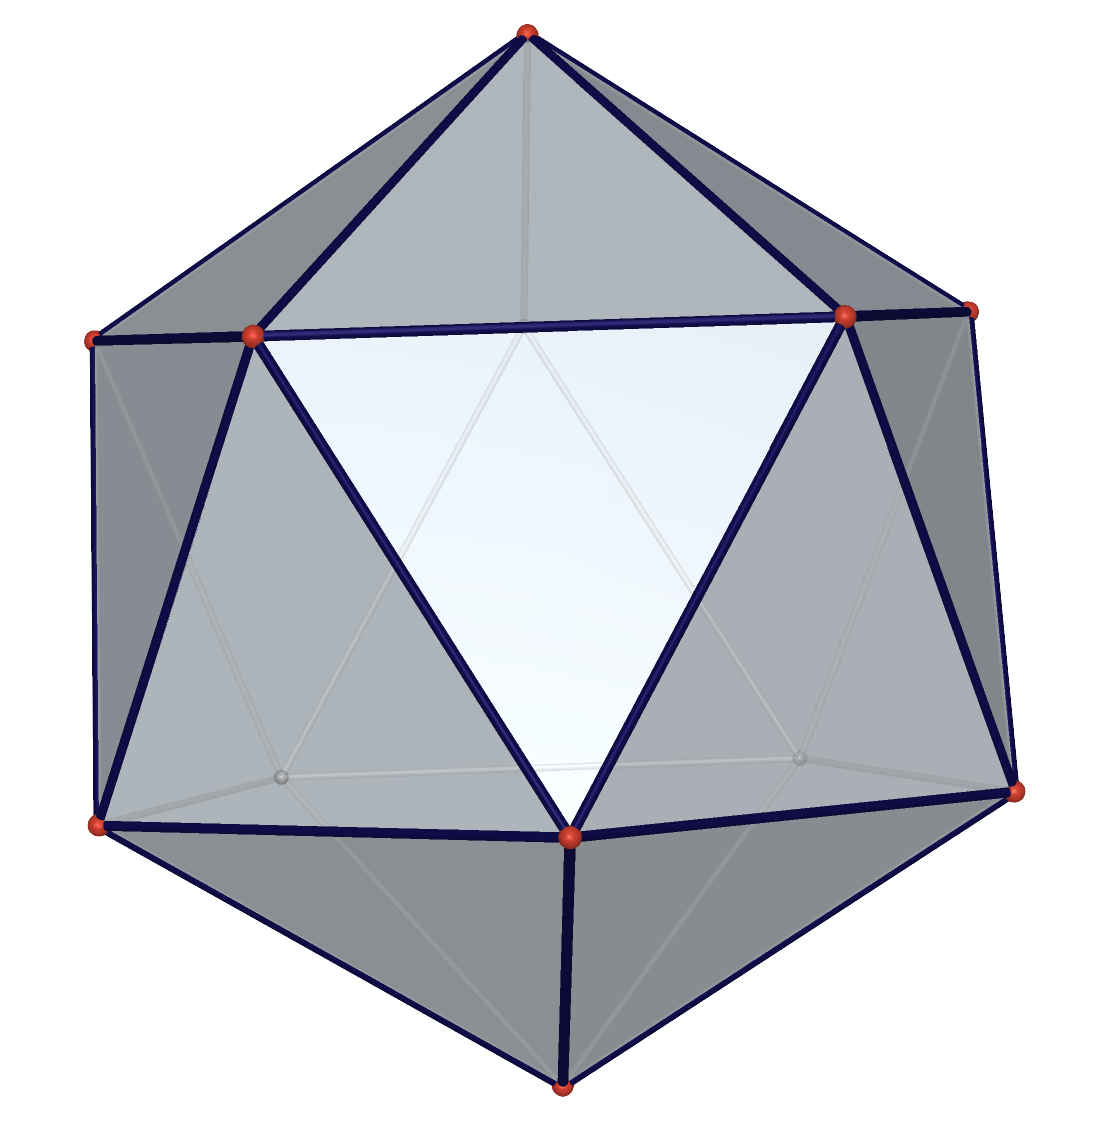
\includegraphics[width=0.15\textwidth]{img-11/icosaedre} \\
			4 triangles &   6 quadrats  & 8 triangles &  12 pentàgons & 20 triangles  \\ \hline
		\end{tabular}
	\end{center}
\end{theorybox}

\begin{comment}
\exer  \includegraphics*[bb=0 0 1.54in 1.20in, width=1.54in, height=1.20in, keepaspectratio=false]{img-11/image6.png}És possible demostrar amb un trencaclosques el teorema de Pitàgores en l'espai. Et proposem que ho intentis. Podràs trobar en la revista i entre els recursos per imprimir les peces que t'ajudaran. En la fotografia es mostra el puzle resolt. 
\end{comment}

%\exer  És possible construir un prisma còncau triangular? I un prisma còncau regular? Raona les respostes.

%\exer  Entre els poliedres regulars, hi ha algun que sigui prisma? En cas afirmatiu classifica-ho.
\begin{mylist}
\exer  És suficient que un paral·lelepípede tingui dues cares rectangulars perquè sigui un prisma recte?
\answers{No. Si les bases són dos rectangles iguals i les cares laterals són romboides es tracta d'un prisma
	oblic.}

\exer  Dibuixa un prisma pentagonal regular i comprova que compleix la relació de Euler.
\answers{ Té set cares, quinze arestes i deu vèrtexs: 7 + 10 =  15 + 2.}

 
\exer \mental  Classifica els següents poliedres convexos en regulars o irregulars


	\begin{longtable}{p{1in}p{1in}p{1in}p{1.0in}p{1in}}
a) 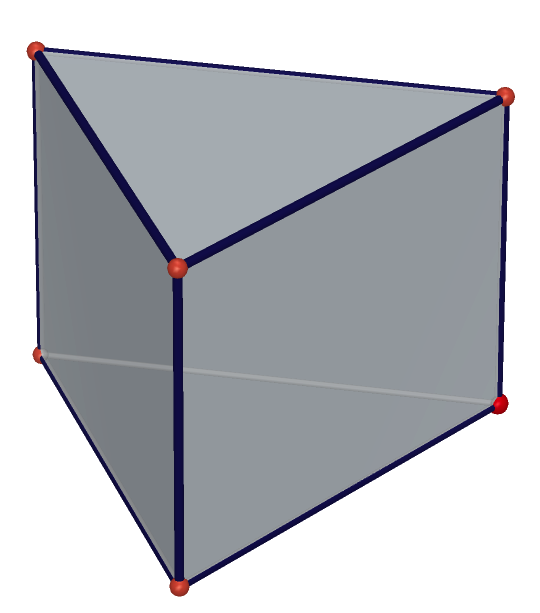
\includegraphics[width=0.8in]{img-11/prisma-triangular} & 
b)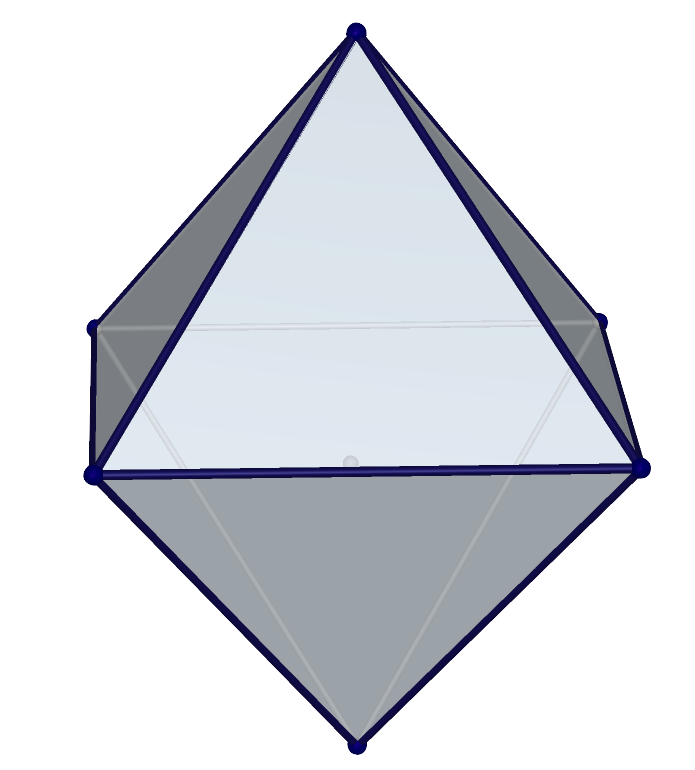
\includegraphics[width=0.8in]{img-11/octaedre} & 
c)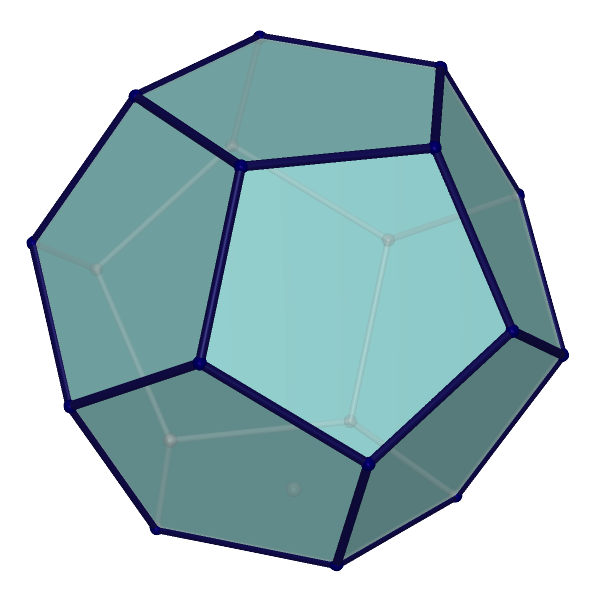
\includegraphics[width=0.8in]{img-11/dodecaedre} & 
d)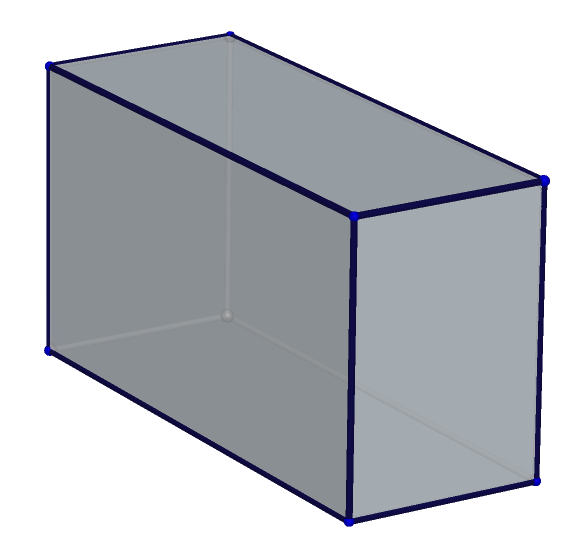
\includegraphics[width=0.78in]{img-11/ortoedre} & 
e) 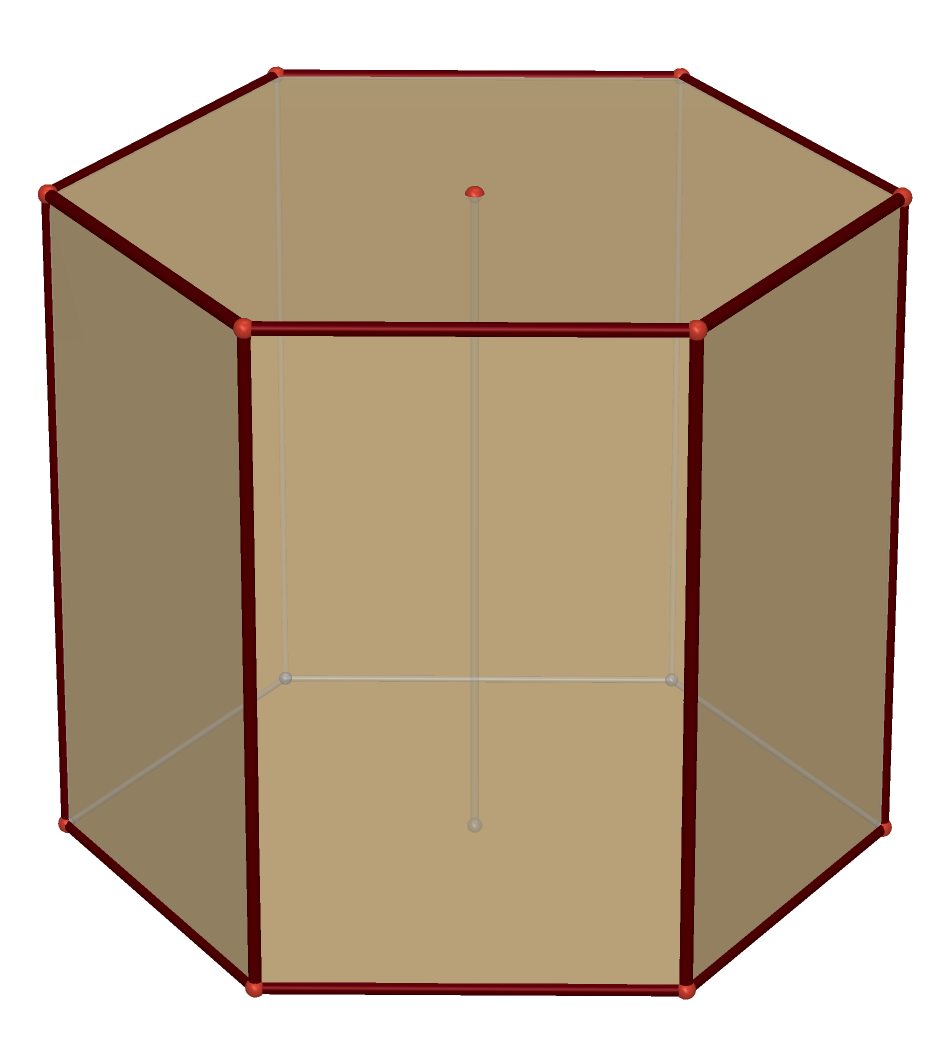
\includegraphics[width=0.7in]{img-11/prisma-hexagonal} \\ 
\end{longtable}
\answers{[Irregular, Regular, Regular, Irregular, Irregular]}

%\exer  Hi ha alguna piràmide regular que sigui poliedre regular? I piràmides amb cares paral·leles? En cas afirmatiu posa un exemple i en cas negatiu, justifica les teves respostes.

\exer  Dibuixa una piràmide hexagonal regular i distingeix l'apotema de la piràmide de l'apotema de la base. Dibuixa també el seu desenvolupament.

\answers{Resposta gràfica:\par 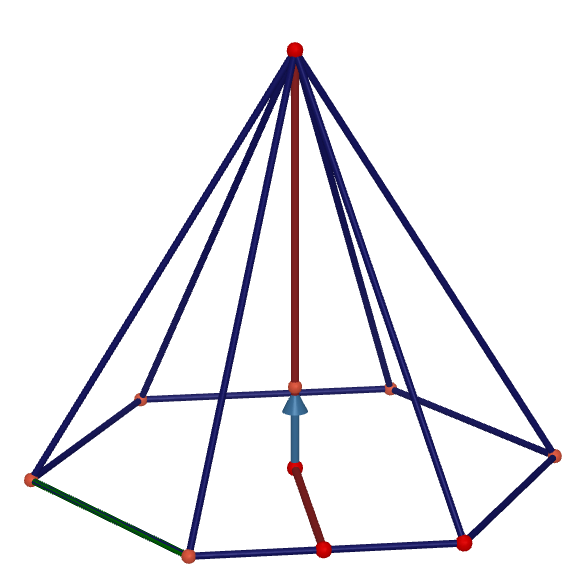
\includegraphics[width=0.4\textwidth]{img-sol/t11-14a}\par 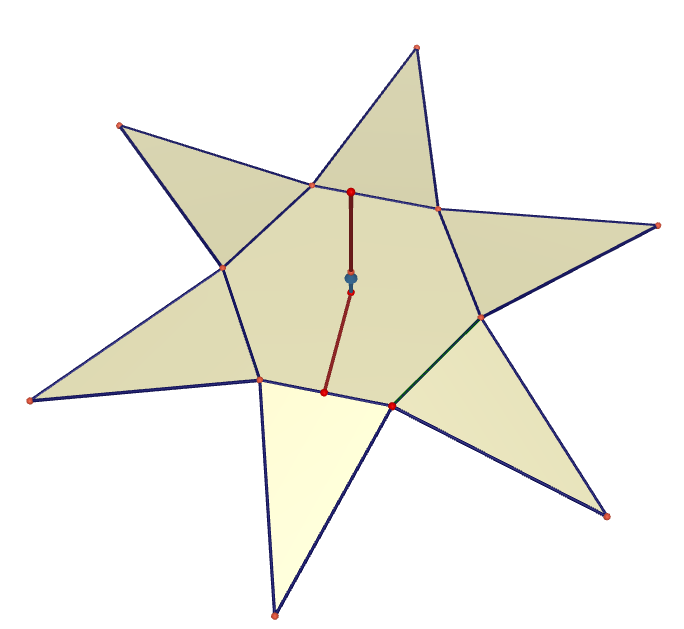
\includegraphics[width=0.4\textwidth]{img-sol/t11-14b}}
 

\end{mylist}
\subsection{Teorema de Pitàgores a l'espai}

\begin{mylist}
\exer[1]  Una caixa té forma cúbica de 2 dm d'aresta. Quant mesura la seva diagonal?
\answers{Teorema de Pitàgores a l'espai:\par $D=\sqrt{2^2+2^2+2^2}=3.46$ dm}

\exer[1]  Calcula la mesura de la diagonal d'una sala que té 10 metres de llarg, 4 metres d'ample i 3 metres d'altura.
\answers{Teorema de Pitàgores a l'espai:\par $D=\sqrt{10^2+4^2+3^2}=11.18$ m}
\end{mylist}
 


\subsection{Àrea lateral i total de poliedres}

\begin{theorybox}
	Trobareu un resum de les fórmules que heu de menester al resum de la pàgina \pageref{sec:resum11}.
\end{theorybox}

\begin{mylist}
	
\exer Calcula les àrees lateral i total d'un prisma triangular regular sabent que les arestes de les bases mesuren 2 cm i cada aresta lateral 8 m. \textbf{Atenció} 8 m = 800 cm!
\answers{$A=4800  + 2 \sqrt{3}$ cm$^2 =   4803,4641$ cm$^2$}

\exer  L'àrea lateral d'un prisma regular de base quadrada és 63 m${}^{2}$ i té 7 m d'altura. Calcula el perímetre de la base.
\answers{El perímetre de la base són 9 m}

\exer  El costat de la base d'una piràmide hexagonal regular és de 6 cm i l'altura de la piràmide 10 cm. Calcula l'apotema de la piràmide i la seva àrea total.
\answers{Apotema = $\sqrt{127}\approx  11,13$ cm; i Àrea = $18 \sqrt{127}+   108\sqrt{3} \approx   389,91$ cm$^2$.}

\vspace{-1cm}
\exer[1]  \begin{minipage}[t]{0.7\textwidth} Calcula l'àrea \underline{lateral} d'un tronc de piràmide regular, sabent que les seves bases són dos octògons regulars de costats 4 i 7 dm i que l'altura de cada cara lateral és de 8 dm. 
	%L'apotema de la base en un octògon és $a_p =1.21 \, c $.
\end{minipage}
\begin{minipage}{0.25\textwidth}
	\vspace{1cm}
	\centering
\includegraphics*[width=2.5cm]{img-11/tronc-octogon.png}
\end{minipage}
\answers{$A_L=352$ cm$^2$}

\exer[1]  \hot Si l'àrea lateral d'una piràmide quadrangular regular és 104 cm${}^{2}$, calcula l'apotema de la piràmide i la seva altura.
 \answers{Totes les arestes mesuren $x=7.75$, l'altura d'una cara lateral $a_P=6.71$ i l'altura de la piràmide $H=5.48$ cm}
 
\end{mylist}


\section{Cossos de revolució}

\begin{theorybox}
	Els cossos de revolució són: El cilindre, el con i l'esfera. Tots ells s'obtenen de fer girar al voltant d'un eix una corba anomenada \textbf{generatriu}.
	\begin{center}
		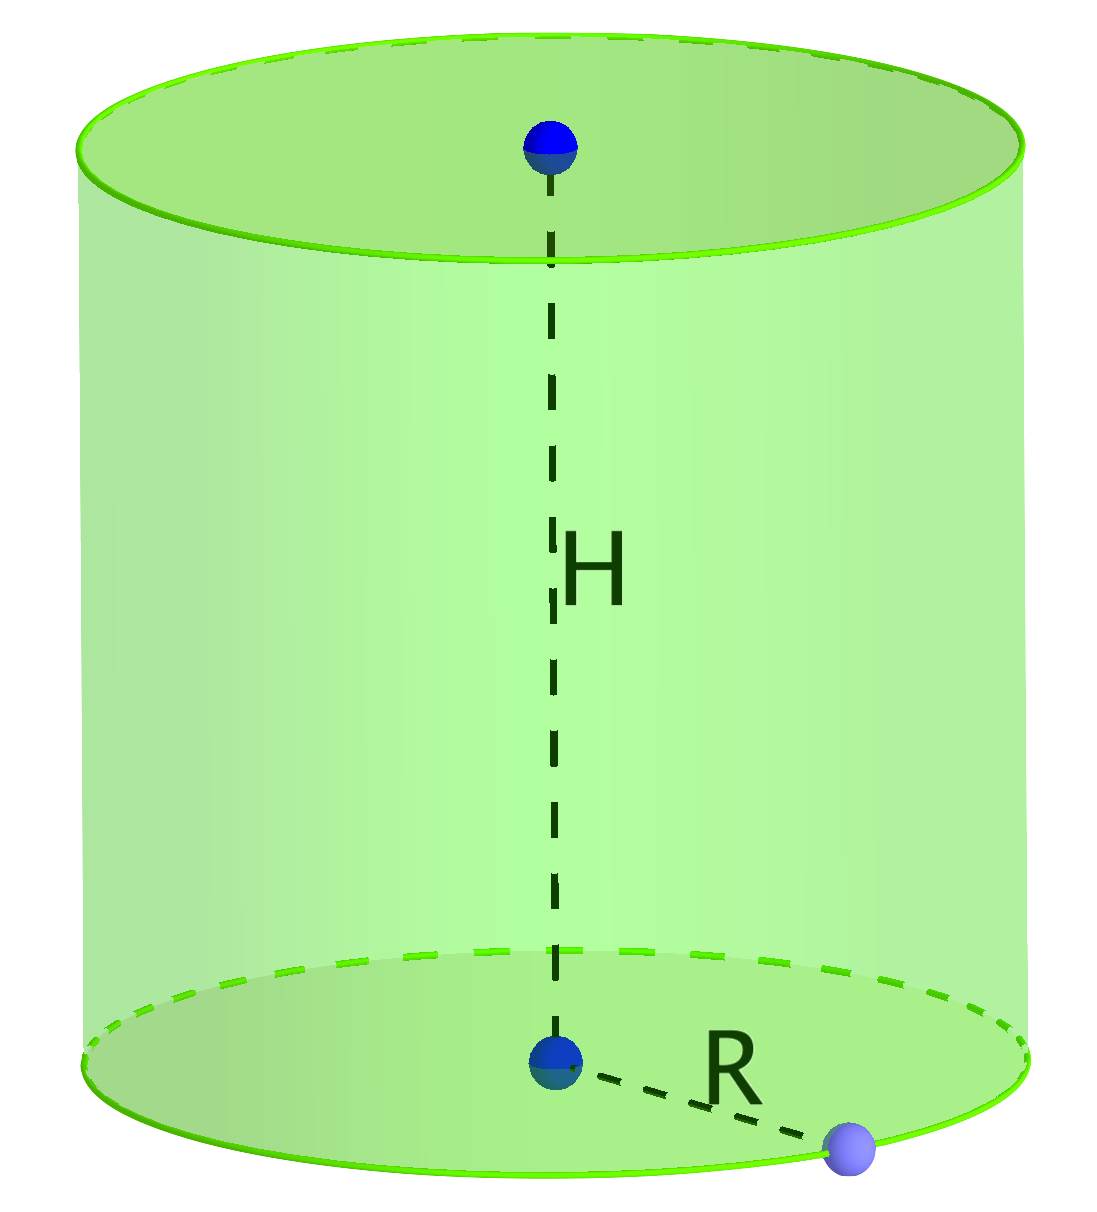
\includegraphics[height=2.5cm]{img-11/cilindro} \quad
			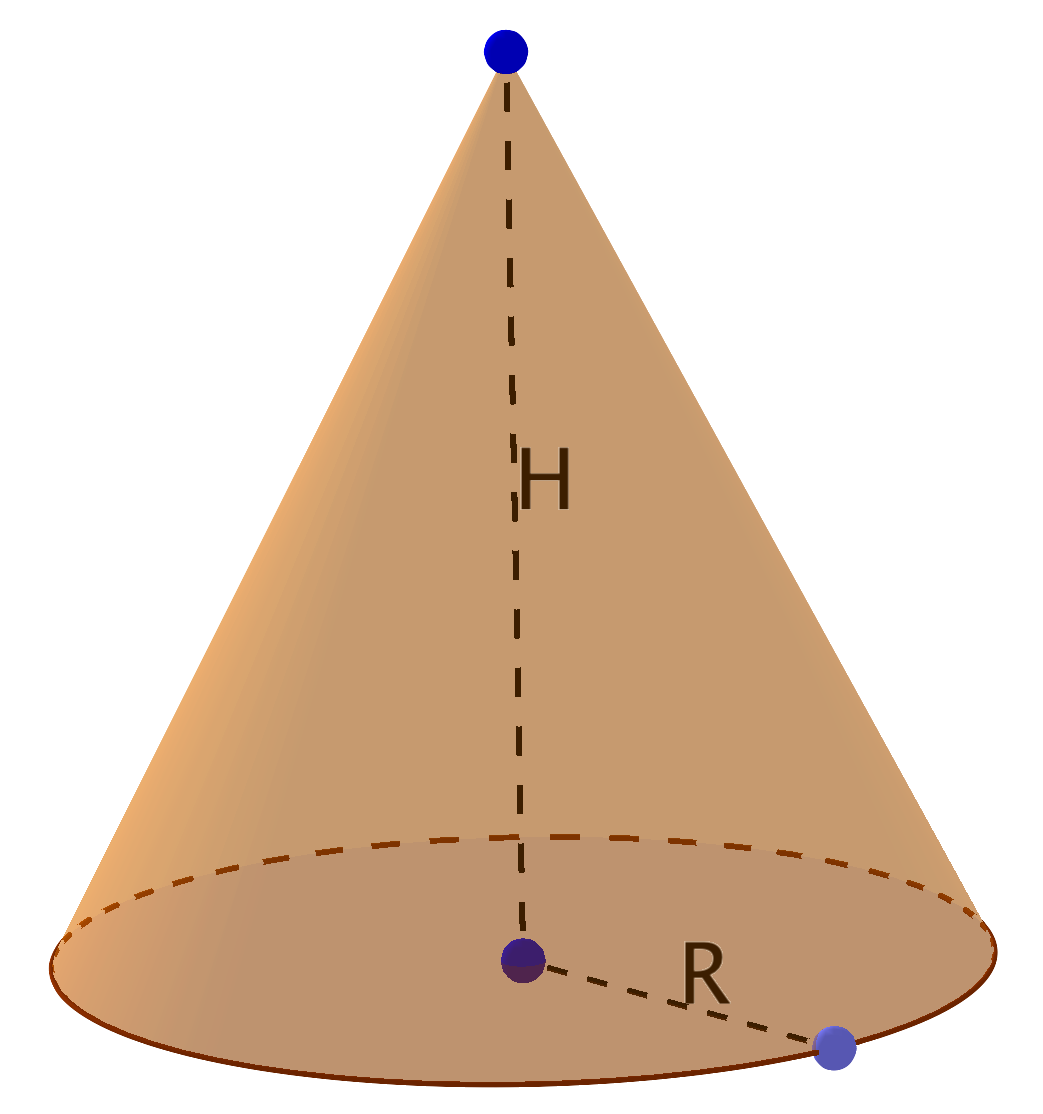
\includegraphics[height=2.5cm]{img-11/cono}  \quad
				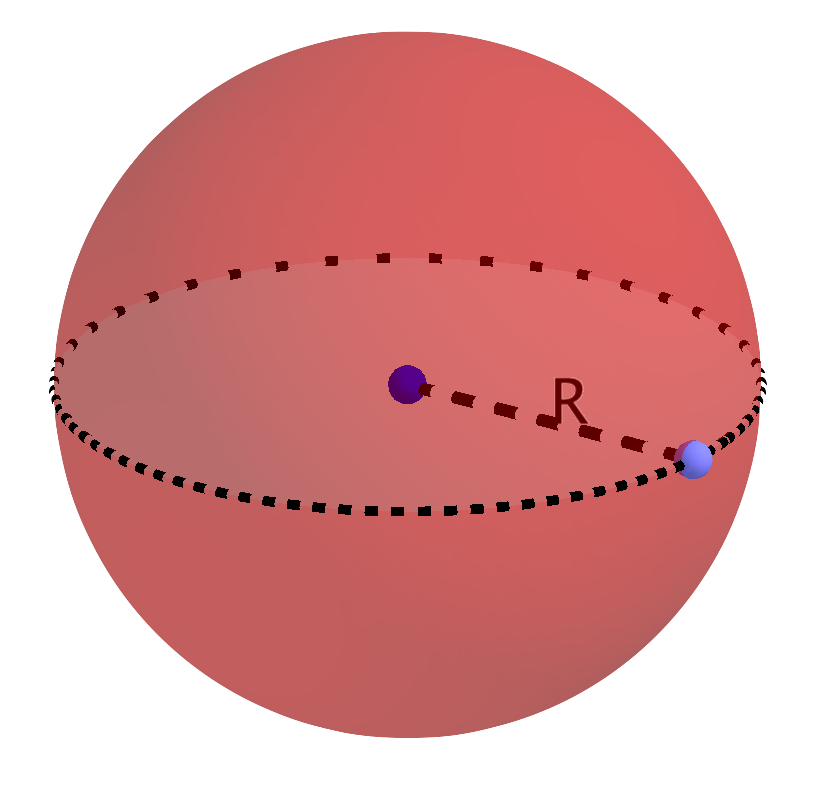
\includegraphics[height=2.5cm]{img-11/esfera} 
	\end{center}
	
\end{theorybox}

\begin{mylist}
\exer Una columna cilíndrica té 76 cm de diàmetre i 4 m d'altura. Quina és la seva àrea lateral?
\answers{$A_L=\frac{76}{25}\pi \approx 9.550442$ m$^2$}

\exer  El radi de la base d'un cilindre és de 38 cm i l'altura és el triple del diàmetre. Calcula la seva àrea total.
\answers{$A_T = 2016 \pi \approx 63510.44$ cm$^2$}

\exer[1]  Calcula l'àrea lateral d'un con recte sabent que la seva generatriu mesura 50 dm i el radi de la base 30 dm.
\answers{$A_L=4712.4$ dm$^2$}

\exer  La circumferència de la base d'un con mesura 6,25 m i la seva generatriu 8 m. Calcula l'àrea total.
\answers{$A_T=\left( \frac{625}{64 \pi} + 25 \right) \approx 28.108495$ m$^2$}

\exer  Una esfera té 4 m de radi. Calcula: a) la longitud de la circumferència màxima; b) l'àrea de l'esfera.
\answers{[$L=8\pi=25.133$ m, $64\pi=201.062$ m$^2$]}

 
\end{mylist}


\section{Volum de cossos geomètrics}

\begin{theorybox}
	Trobareu un resum de les fórmules que heu de menester al resum de la pàgina \pageref{sec:resumvolums}.
\end{theorybox}

\begin{mylist}
\exer Calcula el volum d'un prisma recte de 12 dm d'altura la base de la qual és un hexàgon de 4 dm de costat.
\answers{$V=288\sqrt{3}=408.83$ dm$^3$}

\exer  Calcula la quantitat d'aigua que hi ha en un recipient amb forma de cilindre sabent que la seva base té 12 cm de diàmetre i que l'aigua aconsegueix 1 dm d'altura. 
\answers{$V=360\pi=1130.97$ cm$^3$. En capacitat $1$ dm$^3$=1 l, llavors aprox. 1,13 litres.}

\exer[1]  El dipòsit de gasoil de la casa d'Irene és un cilindre d'1 m d'altura i 2 m de diàmetre. Irene ha cridat al subministrador de gasoil perquè en el dipòsit només hi queden 140 litres.

\begin{tasks}
   \task Quin és, en dm${}^{3}$, el volum del dipòsit? (Utilitza 3,14 com a valor de $\pi$).
   \task Si el preu del gasoil és de 0,80 \euro{} per litre, quant haurà de pagar la mare d'Irene per omplir el dipòsit?
\end{tasks}
\answers{[$V=1000\pi=3140$ dm$^3$=litres, costarà 2400 \euro{}]}

\exer   Comprova que el volum de l'esfera de radi 5 dm sumat amb el volum d'un con del mateix radi de la base i 10 dm d'altura, coincideix amb el volum d'un cilindre que té 10 dm d'altura i 5 dm de radi de la base. 
\answers{Els dos volums són iguals a $\frac{500 \pi}{3}=523.6$ dm$^3$}

\end{mylist}
 


\section{Globus terraqüi}

\begin{mylist}
\exer Un avió recorre 20${}^\circ$ en direcció Oest al llarg de l'Equador. Si arriba a un punt la longitud del qual és de 170${}^\circ$Est, quines són les coordenades del lloc de partida?

\answers{$0^\circ$ de latitud i $170^\circ$ Oest}

\exer  Joan surt de la seva casa i recorre 10 km en direcció sud, 20 km cap a l'est i 10 km cap al nord. Si es troba de nou a casa, on està situada la seva casa?

\answers{En el pol nord exactament}

\exer  En l'esfera terrestre, quin paral·lel mesura més?, quin meridià mesura més? Raona les teves respostes.

\answers{El paral·lel major és l'equador. Tots els meridians són iguals (si menyspream el fet que la Terra no sigui perfectament esfèrica; clar).}

\exer  Cerca les coordenades geogràfiques del lloc en el qual vius.


\begin{center}
 \includegraphics*[width=12cm]{img-11/planisferi.png} 
\end{center} 

\answers{Binissalem: Latitud=39.688035${}^\circ$ Nord; Longitud=2.8439975${}^\circ$ Est}
 
\end{mylist}



\begin{activitats}


\subsection{Angles polièdrics. Paral·lelisme i perpendicularitat. Poliedres.}

\begin{mylist}


\exer Si estem en una habitació sense columnes, atenent al terra i a les seves quatre parets, quants angles diedres es formen?
\answers{Dotze diedres si l'habitació té sòtil. 8 sense sòtil.}

\exer  Doblega per la meitat un full de paper, construeix un angle diedre i traça el seu rectilini. Podries mesurar l'amplitud de diferents angles diedres mitjançant aquest rectilini?
\answers{Solució oberta i manipulativa}

\exer  Determina l'amplitud dels angles diedres que formen les cares laterals d'un poliedre que és un prisma recte de base un octògon regular.
\answers{135$^\circ$}

\exer  Dues cares d'un triedre mesuren 60${}^\circ$ i 118${}^\circ$, Entre quins valors pot oscil·lar l'altra?
\answers{Entre 0$^\circ$ i 182$^\circ$, ambdós exclosos}

\exer  Es pot formar un angle poliedre amb un angle d'un triangle equilàter, dos d'un rectangle i un d'un pentàgon regular?
\answers{Sí es pot. $60^\circ + 2 \cdot 90^\circ + 108^\circ = 348^\circ < 360^\circ$}

\exer  Podrà existir un poliedre regular que les seves cares siguin hexagonals? Raona la resposta.
\answers{No es pot. $120^\circ \cdot 3 = 360^\circ$}

\exer  Quantes diagonals pots traçar en un cub? I en un octàedre?
\answers{En un cub 4, en un octaedre 3}

\exer  Pots trobar dues arestes paral·leles en un tetraedre? I en cadascun dels restants poliedres regulars?
\answers{En el tetraedre no. En tots els demés, sí}

\exer  Perllonga una parella d'arestes en una piràmide pentagonal, de manera que s'obtinguin rectes no coplanàries.
\answers{Solució oberta\par
	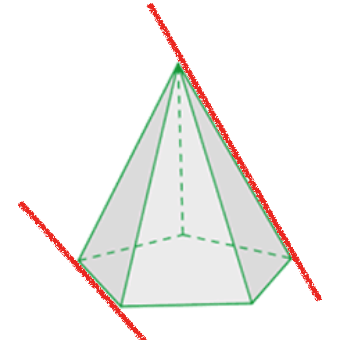
\includegraphics[width=0.45\textwidth]{img-sol/t11-41}}

\exer  Dibuixa un prisma regular de base quadrada i assenyala: a) dues arestes que siguin paral·leles, b) dues arestes que siguin perpendiculars i coplanàries, c) dues arestes perpendiculars i no coplanàries, d) dues cares paral·leles, e) dues cares perpendiculars.
\answers{Solució gràfica: \par 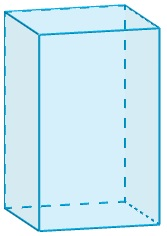
\includegraphics[width=0.45\textwidth]{img-sol/prisma-cuadrangular}}

\exer  Si un poliedre convex té 16 vèrtexs i 24 arestes, quantes cares té? Podria ser una piràmide? I un prisma?
\answers{Ha de tenir 20 cares. Una piràmide convexa té tantes cares com vèrtexs, així que no pot ser una piràmide. Un prisma convex de 20 cares tindria dues bases i 18 cares laterals. En aquest cas hauria 54 arestes i 36 vèrtexs.}

\exer  Amb 12 varetes de 5 cm de llarg cadascuna, usant totes les varetes quins poliedres regulars es poden construir?
\answers{Es pot construir un cub, un octàedre o dos tetraedres}

\exer  D'un prisma sabem que el nombre de vèrtexs és 16 i que el nombre d'arestes és 24, quantes cares té?
\answers{Té 10 cares. És un prisma octogonal.}

\exer  Classifica els següents cossos geomètrics i indica, quan siguin poliedres, el nombre de vèrtexs, cares i arestes que tenen. Quins compleixen el teorema de Euler?
\begin{tasks}(2) 
\task 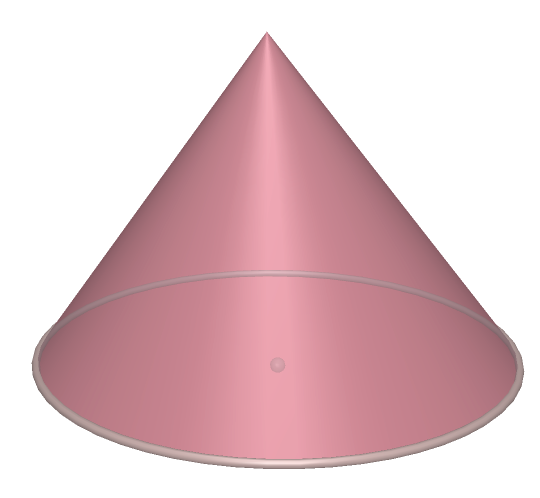
\includegraphics[width=1in]{img-11/con}
\task 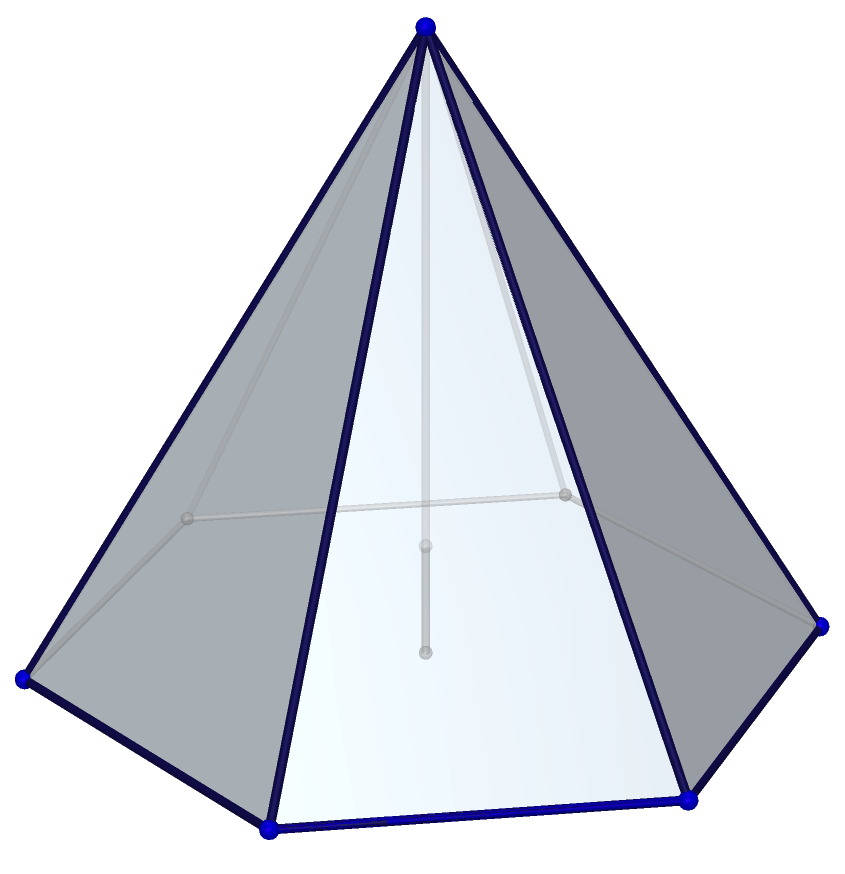
\includegraphics[width=1in]{img-11/piramide-hexagonal}
\task 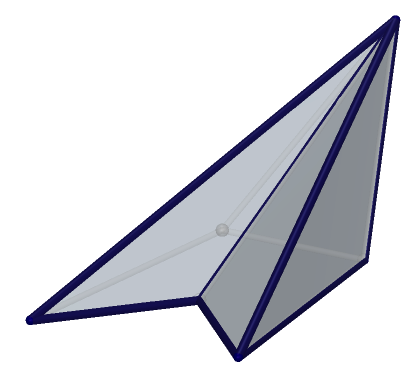
\includegraphics[width=1in]{img-11/poliedre11}
\task 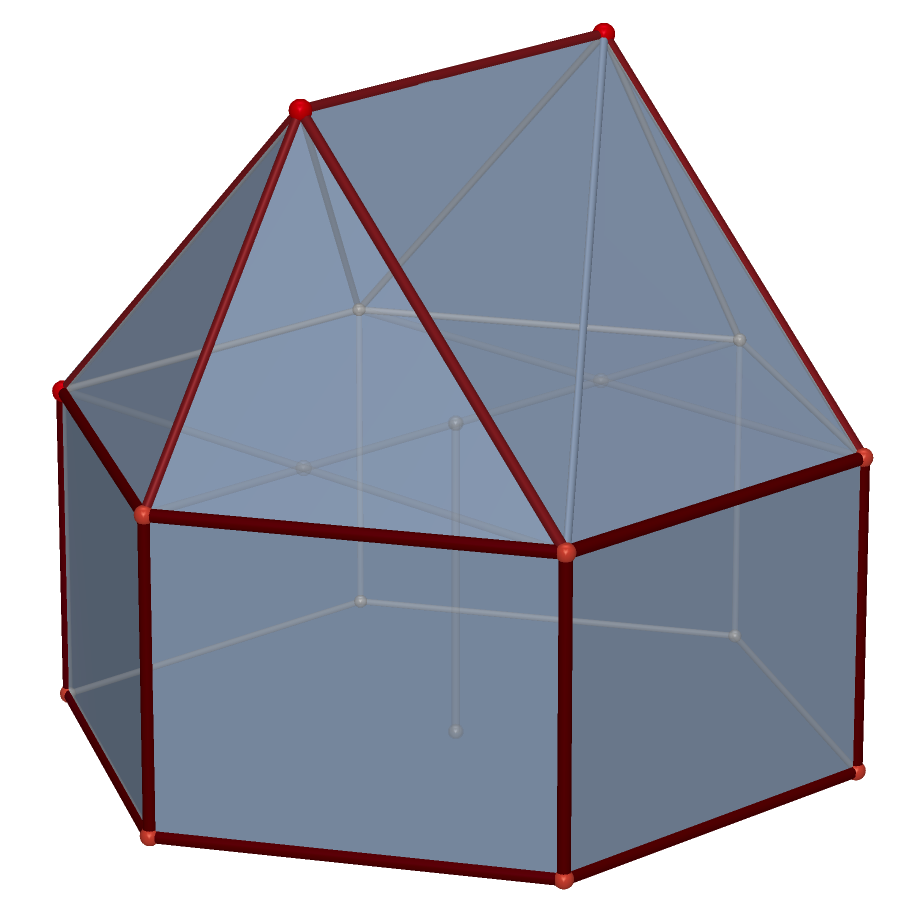
\includegraphics[width=1in]{img-11/raro}
%\task \includegraphics*[bb=0 0 0.58in 0.72in, width=0.58in, height=0.72in, keepaspectratio=false]{img-11/image18.png} 
\end{tasks}
\answers[cols=1]{Con, Piràmide hexagonal regular. Compleix Euler, Piràmide pentagonal còncava. Compleix Euler, Poliedre format per 13 cares; 14 vèrtexs; 19 arestes. Compleix Euler}

\exer  Descriu la diferència entre un prisma recte i un prisma oblic. És suficient que un paral·lelepípede tingui dues cares paral·leles rectangulars perquè sigui un ortoedre?

\answers{En un prisma recte totes les cares laterals són rectangles; en l'oblic algunes no els són.
	Un prisma amb base un rombe o un romboide té quatre cares laterals que són rectangles paral·lels dos a dos i no és un ortoedre.}
 
\end{mylist}

\columnbreak
\subsection{Teorema de Pitàgores en l'espai}

\begin{mylist}
\exer Dibuixa un paral·lelepípede les arestes del qual mesurin 4 cm, 5 cm i 6 cm que no sigui un ortoedre. Dibuixa també el seu desenvolupament.

\answers{Solució gràfica oberta}

\exer  Si el paral·lelepípede anterior fos un ortoedre, quant mesuraria la seva diagonal? 

\answers{$D=\sqrt{4^2+5^2+6^2}=8.77$ cm}

\exer  Un tassó de 12 cm d'altura té forma de tronc de con en el qual els radis de les bases són de 5 i 4 cm. Quant ha de mesurar com a mínim una cullereta perquè sobresurti del tassó almenys 2 cm?

\begin{center}
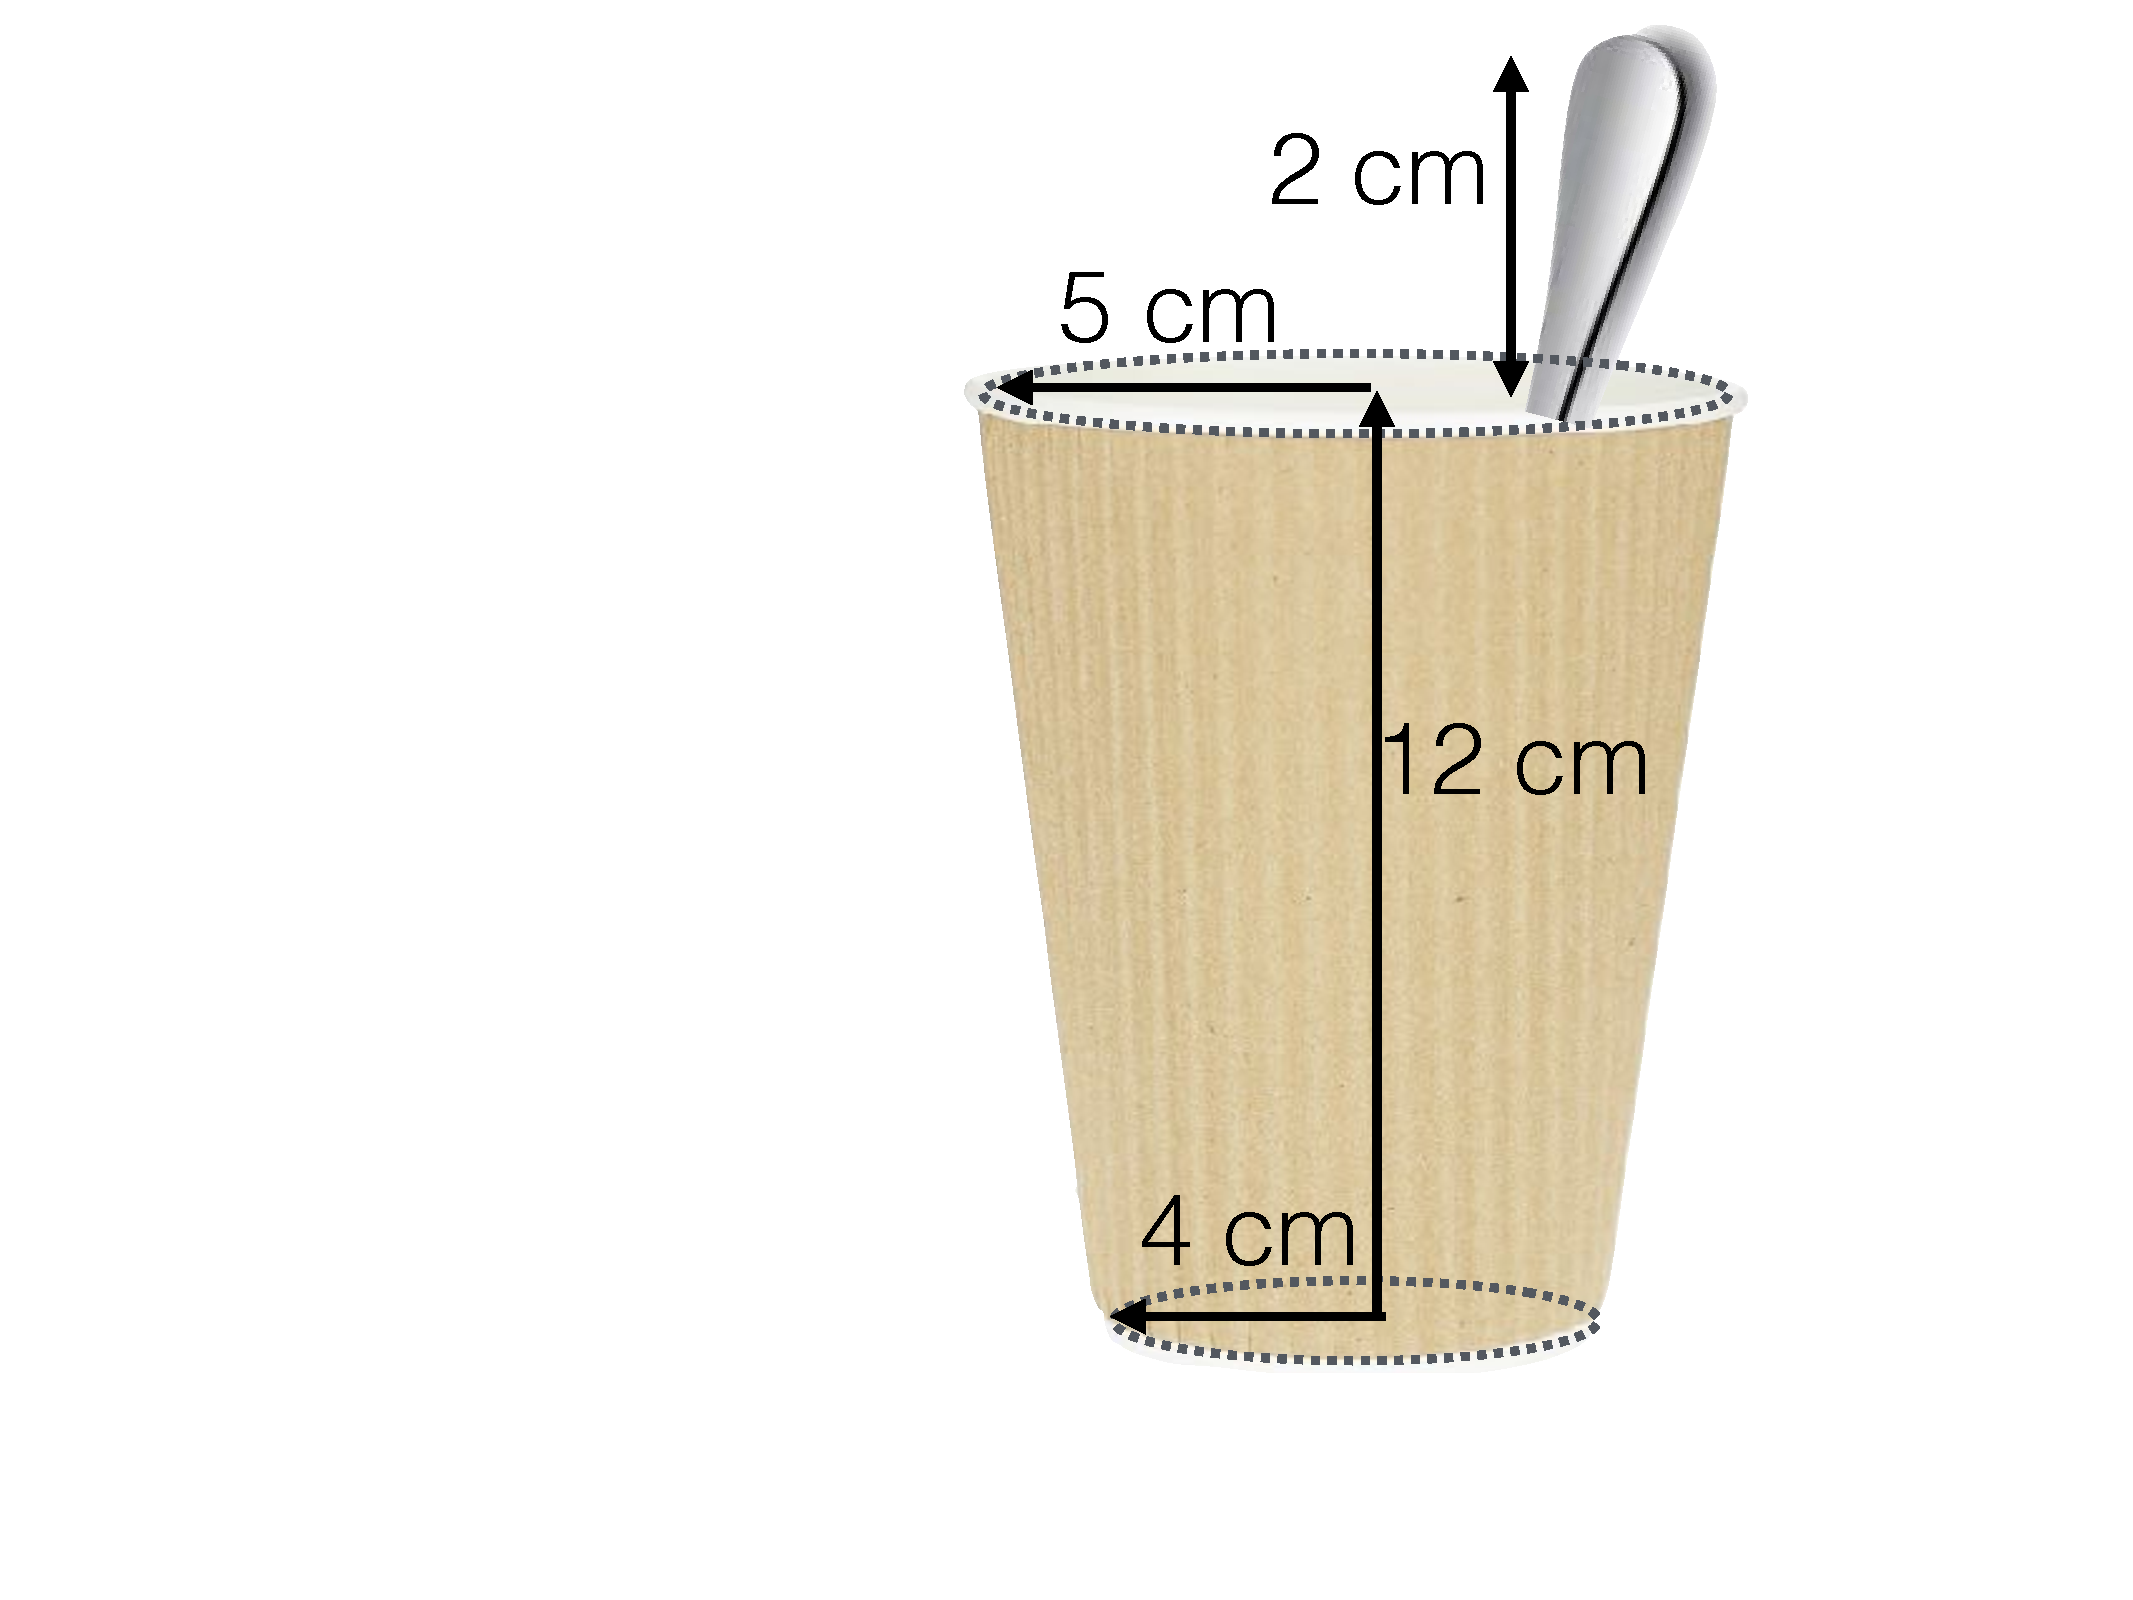
\includegraphics[width=3cm]{img-11/tasso}
\end{center}

\answers{17 cm}

\exer  És possible guardar en una caixa amb forma de ortoedre d'arestes 4 cm, 3 cm i 12 cm un bolígraf de 13~cm de longitud?


\answers{La diagonal d'aquest ortoedre mesura 13 cm. Si el bolígraf té diàmetre diferent de zero en les seves dues extrems, no hi cap.}

\exer  Calcula la diagonal d'un prisma recte de base quadrada sabent que el costat de la base mesura 6 cm i l'altura del prisma 8 cm.

\answers{$D=2\sqrt{34}=11.7$ cm}

\exer  Si un ascensor mesura 1 m d'ample, 1,5 m de llarg i 2,2 m d'altura, és possible introduir en ell una escala de 3 m d'altura?

\answers{La diagonal de l'ortoedre mesura aproximadament 2.844 m. L'escala no hi cap.}

\exer  Quin és la major distància que es pot mesurar en línia recta en una habitació que té 6 m d'ample, 8 m de llarg i 4 metres d'altura?

\answers{$2\sqrt{29}=10.77$ m}

\exer  Calcula la longitud de l'aresta d'un cub sabent que la seva diagonal mesura 3,46 cm.

\answers{Aproximadament 2 cm}

\exer  Calcula la distància màxima entre dos punts d'un tronc de con les bases del qual tenen radis 5 cm i 2 cm, i altura 10 cm.

\answers{$\sqrt{149}=12.2$ cm} 
 
 
\end{mylist}

\subsection{Àrea lateral, total i volum de cossos geomètrics}
 
\begin{mylist}
\exer Identifica a quin cos geomètric pertanyen els següents desenvolupaments:


a)  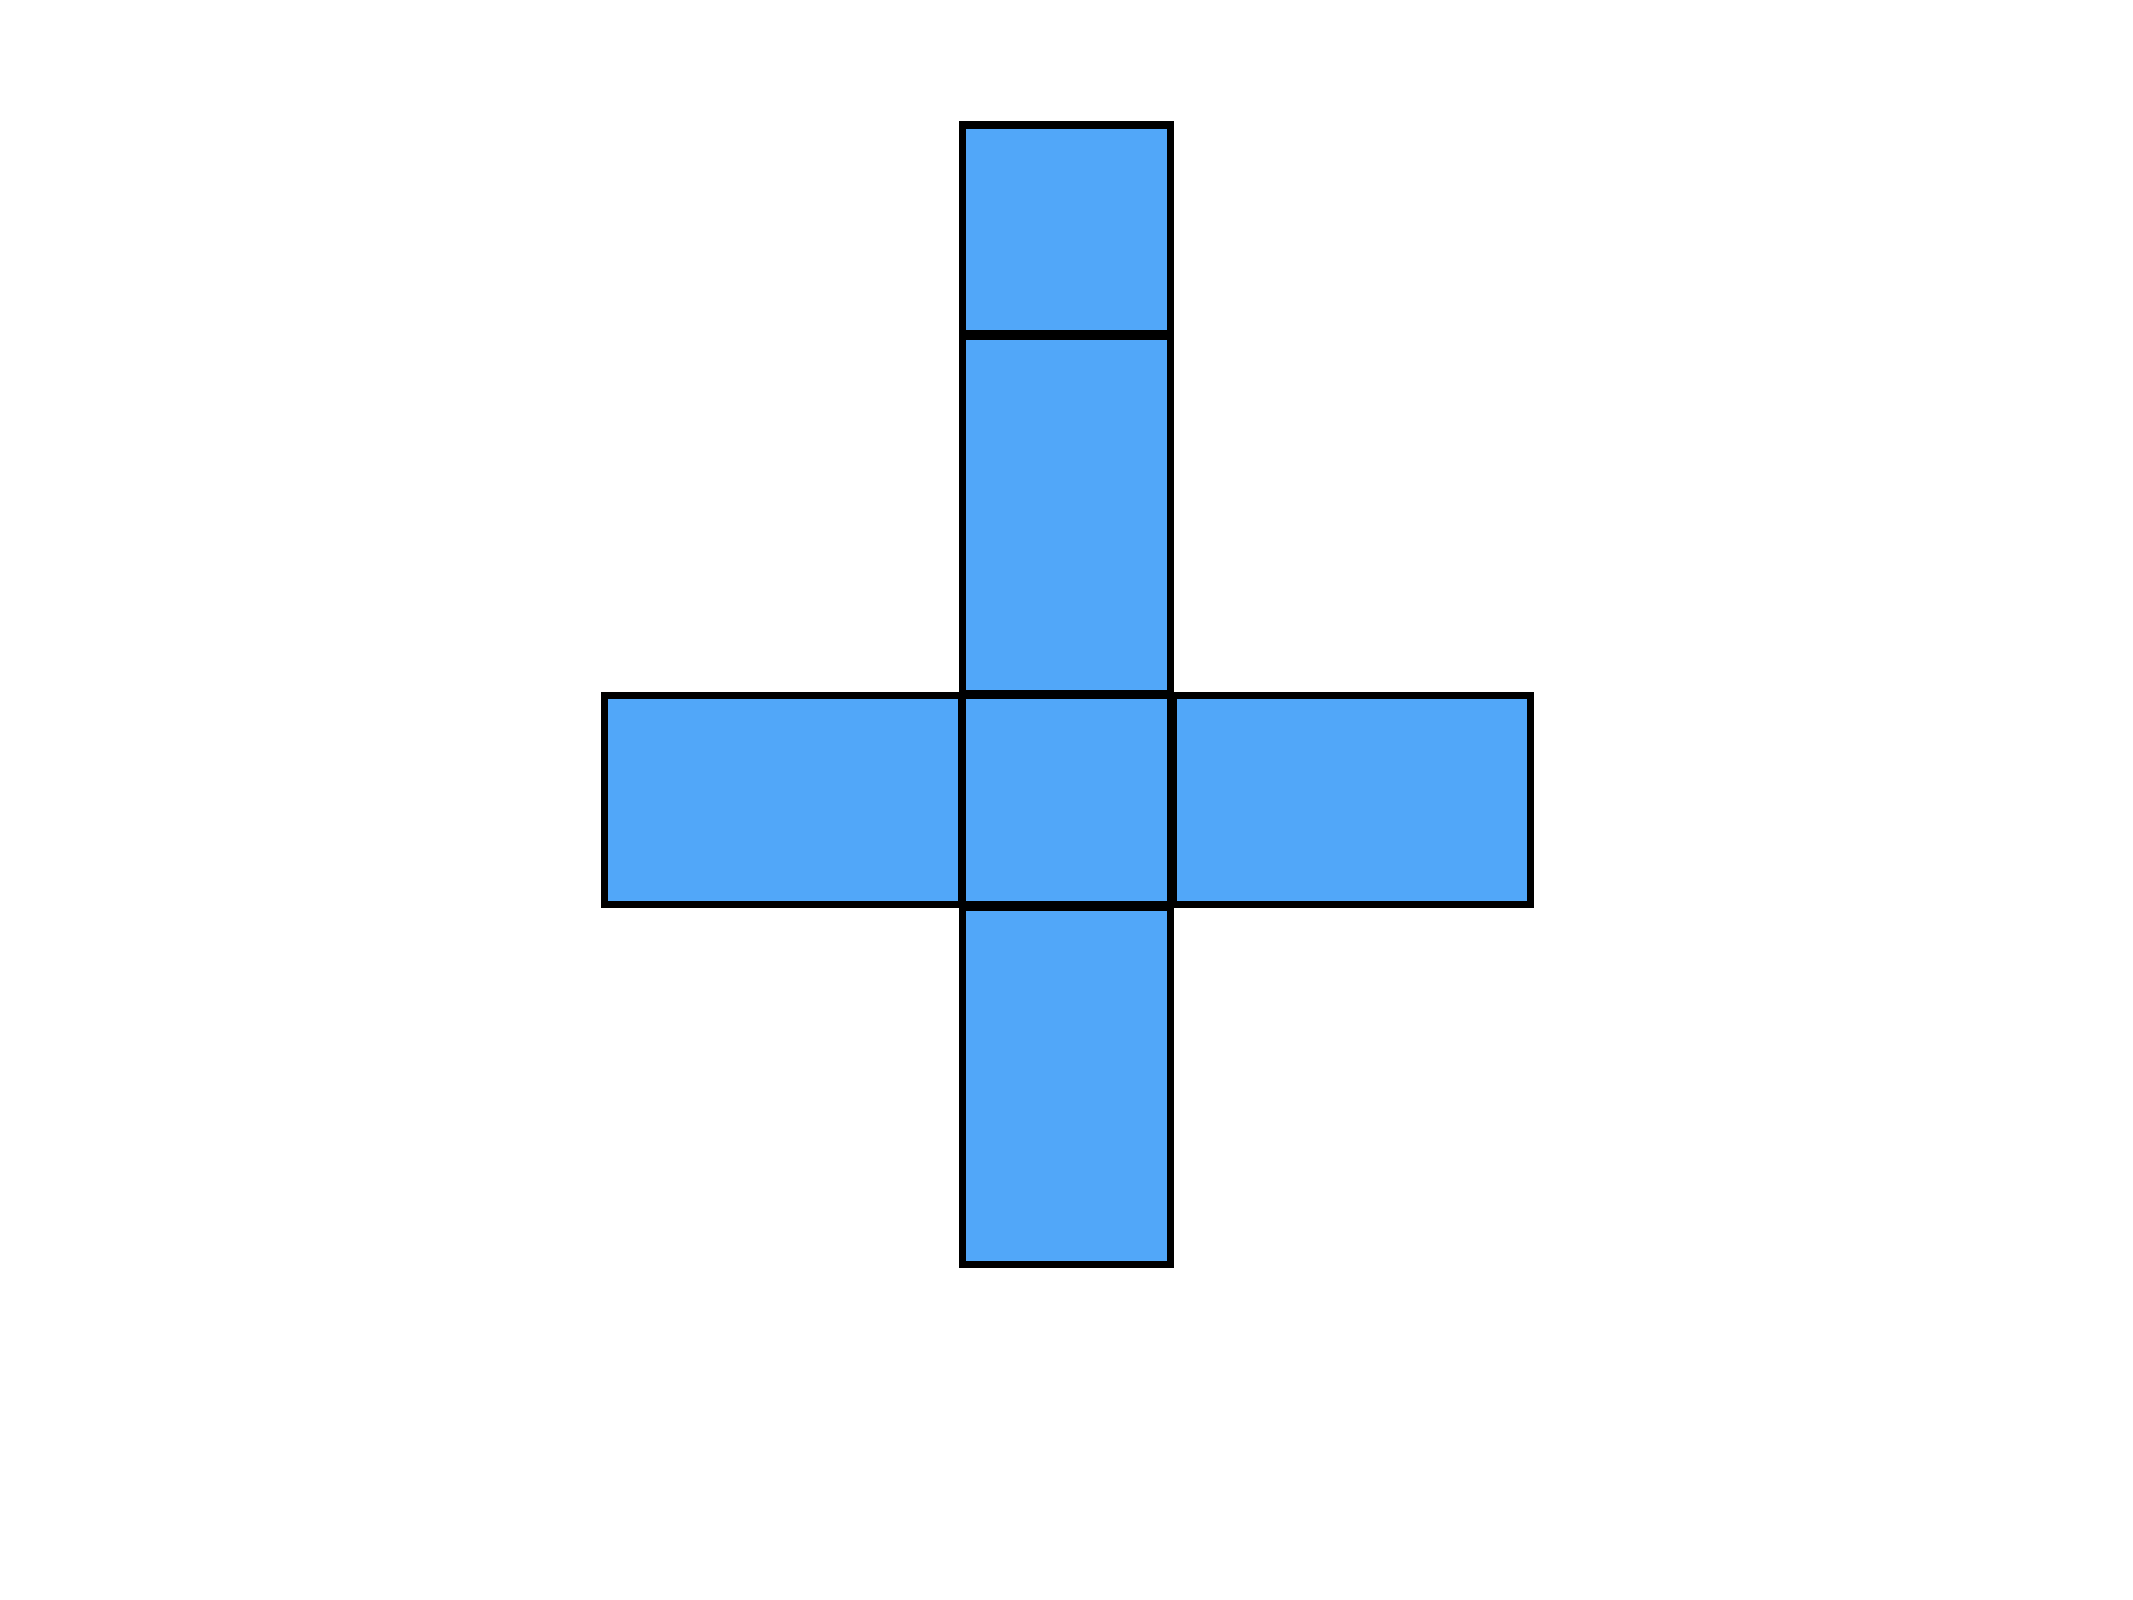
\includegraphics[height=2.2cm]{img-11/desenvolupa1}
b) 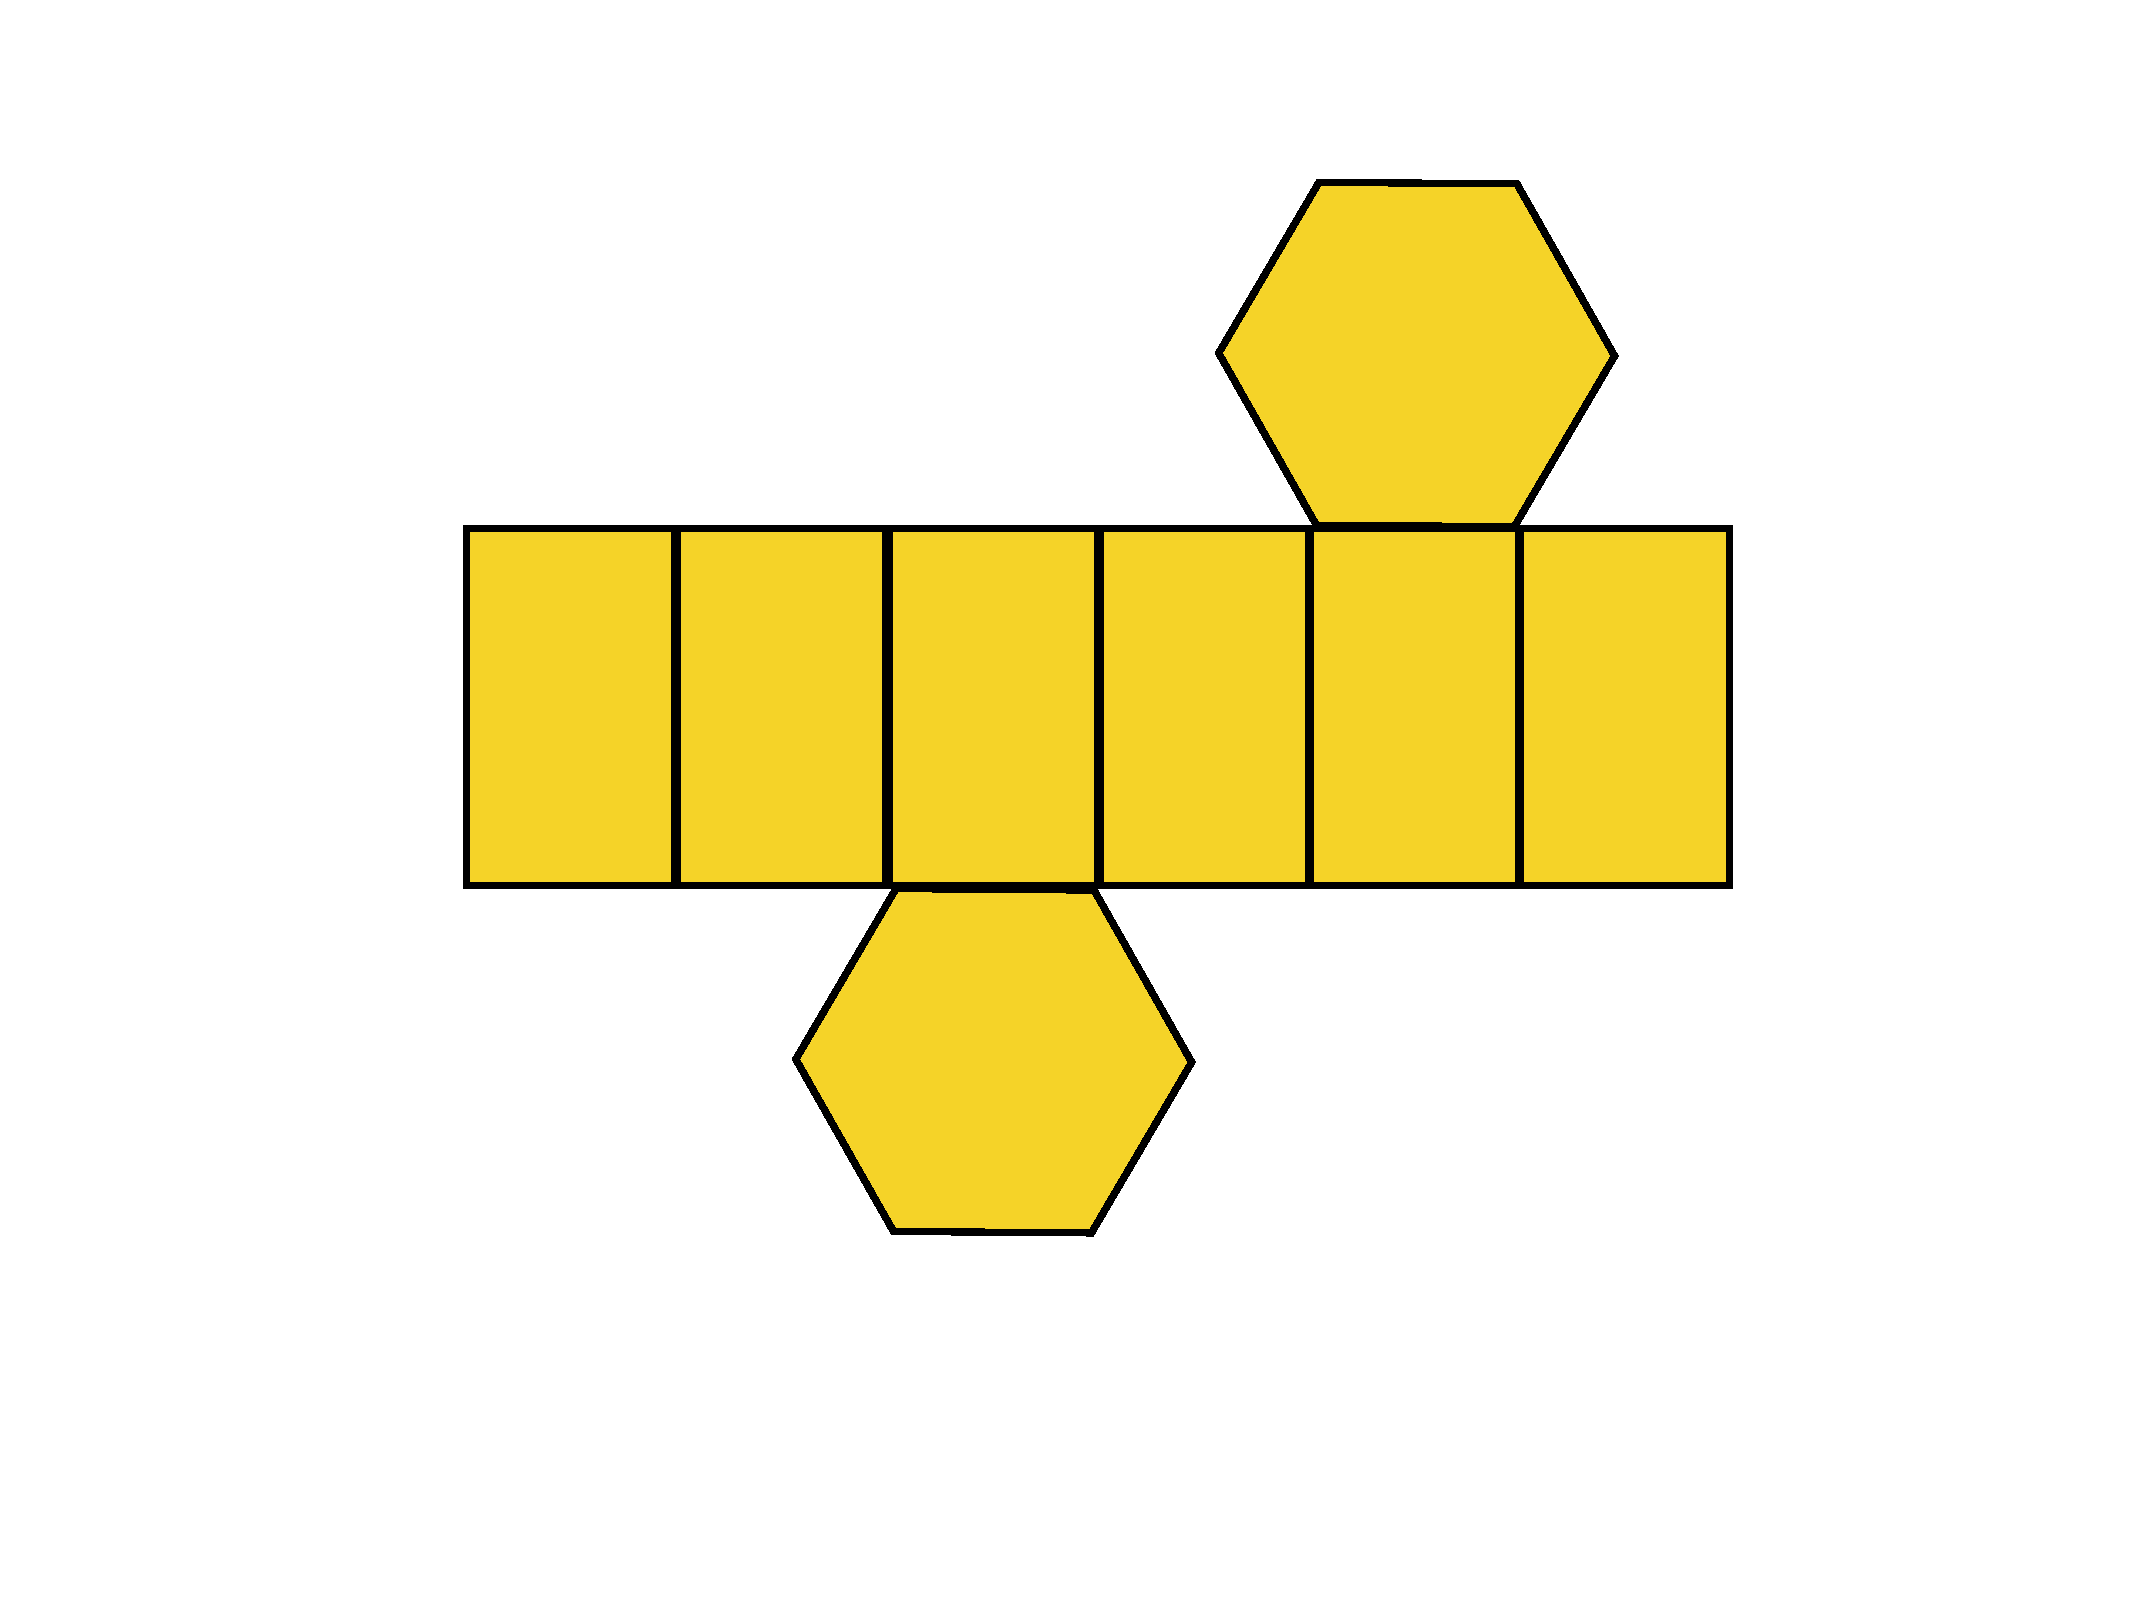
\includegraphics[height=2.2cm]{img-11/desenvolupa2}

c)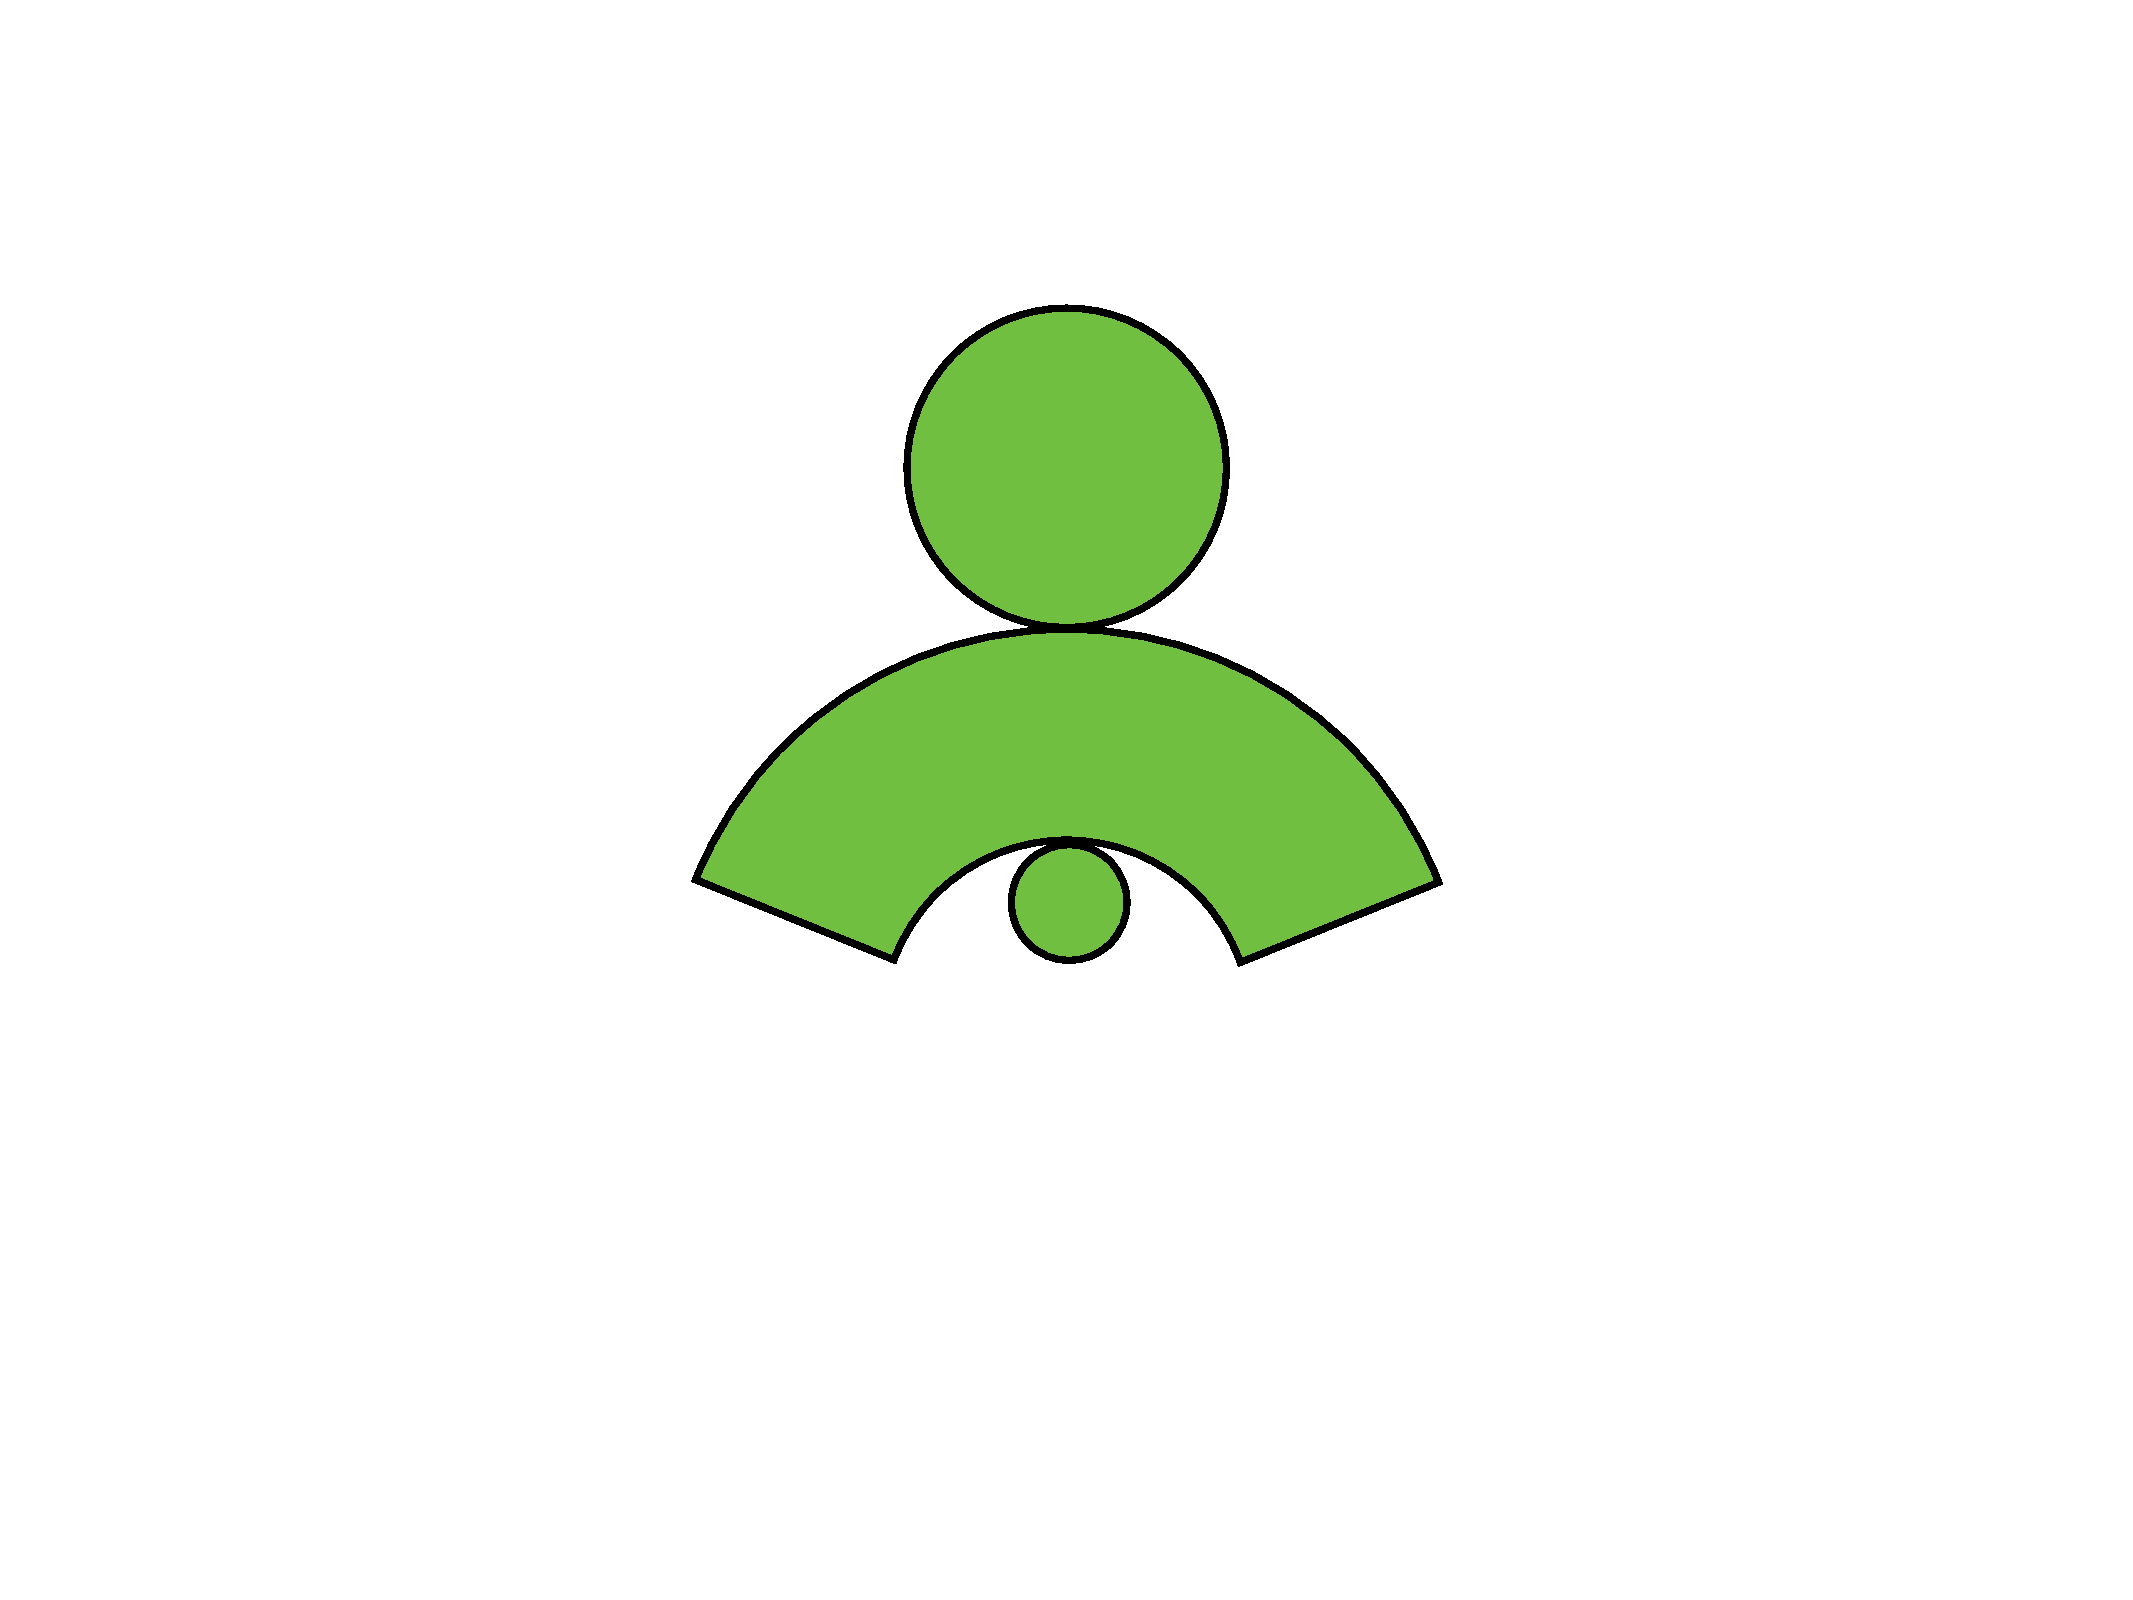
\includegraphics[height=2.2cm]{img-11/desenvolupa3}
d)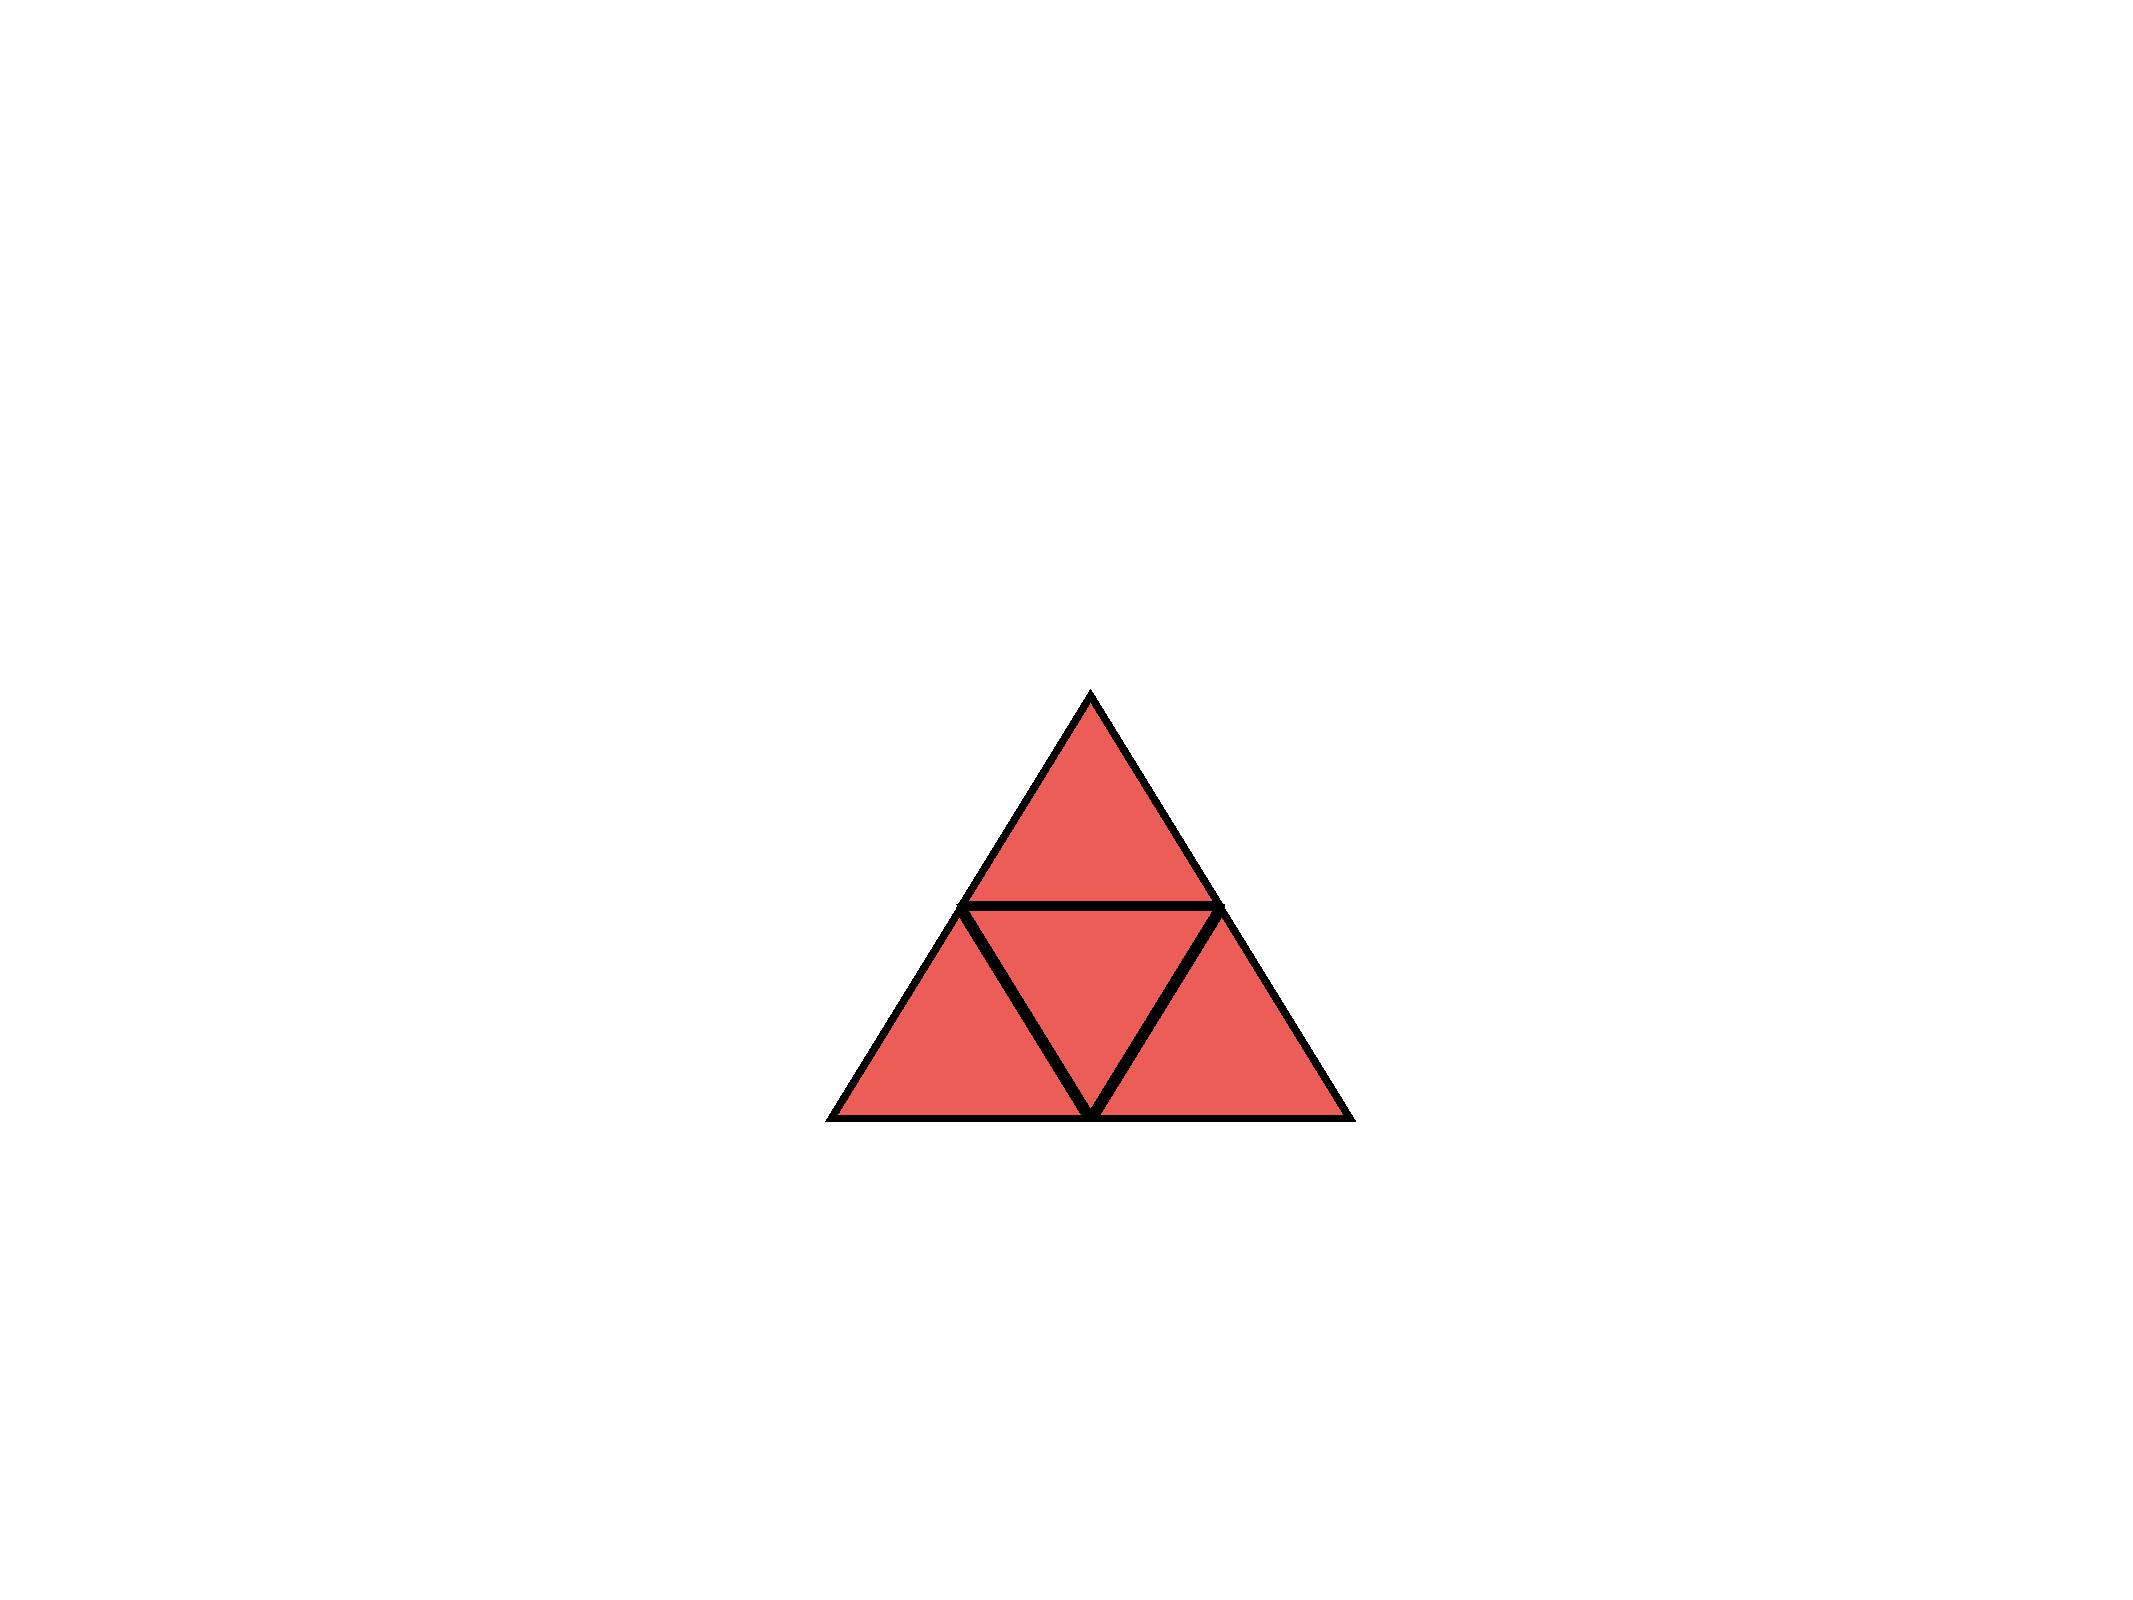
\includegraphics[height=2.2cm]{img-11/desenvolupa4}
% \includegraphics*[bb=0 0 0.72in 0.79in, width=0.72in, height=0.79in, keepaspectratio=false]{img-11/image26.png} \\ \hline 
 
\answers[cols=1]{[Prisma quadrangular regular, Prisma hexagonal regular, Tronc d'un con, Tetraedre]}

\exer  Un prisma de 8 dm d'altura té com a base un triangle rectangle de catets 3 dm i 4 dm. Calcula les àrees lateral i total del prisma.

\answers{$A_L=96$ dm$^2$ i $A_T=108$ dm$^2$}

\exer  Dibuixa un prisma hexagonal regular que tingui 4 cm d'aresta basal i 1 dm d'altura i calcula les àrees de la base i total.

\answers{$A_B=24\sqrt{3}=41.57$ i $A_T=48(5+\sqrt{3})=323.14$ cm$^2$}

\exer  Un prisma pentagonal regular de 12 cm d'altura té una base de 30 cm${}^{2}$ d'àrea. Calcula el seu volum.

\answers{$V=360$ cm$^3$}

\exer  Calcula l'àrea total d'un ortoedre de dimensions 3.5 dm, 8.2 dm i 75 cm.

\answers{$A_T=232.9$ dm$^2$}

\exer  Calcula la superfície total i el volum d'un cilindre que té 8 m d'altura i 5 cm de radi de la base.

\answers{Atenció passa l'altura a cm! $A_T=8950\pi=28\,117.25$ cm$^2$ i $V=20\,000\pi=62\,831.85$ cm$^3$}

\exer  Calcula l'àrea total d'una esfera de 5 cm de radi.

\answers{$A_T=100\pi=314.16$ cm$^2$}

\exer  Calcula l'apotema d'una piràmide hexagonal regular sabent que el perímetre de la base és de 32~dm i l'altura de la piràmide és de 4 dm. Calcula també l'àrea total i el volum d'aquesta piràmide.

\answers{$a_{piram}=\frac{4\sqrt{21}}{3}=6.11$ dm. $A_T=171.66$ dm$^2$; $V=\frac{512\sqrt{3}}{9}=98.53$ dm$^3$. On s'ha calculat també l'apotema de la base $a_{base}=4.6188$ dm i l'àrea de la base $A_B=73.9008$  dm$^2$}

\exer[1]  Calcula l'apotema d'una piràmide regular sabent que la seva àrea lateral és de 120 m${}^{2}$ i la seva base és un hexàgon de 5 m de costat.
\answers{Apotema piràmide 4 m}

\begin{center}
	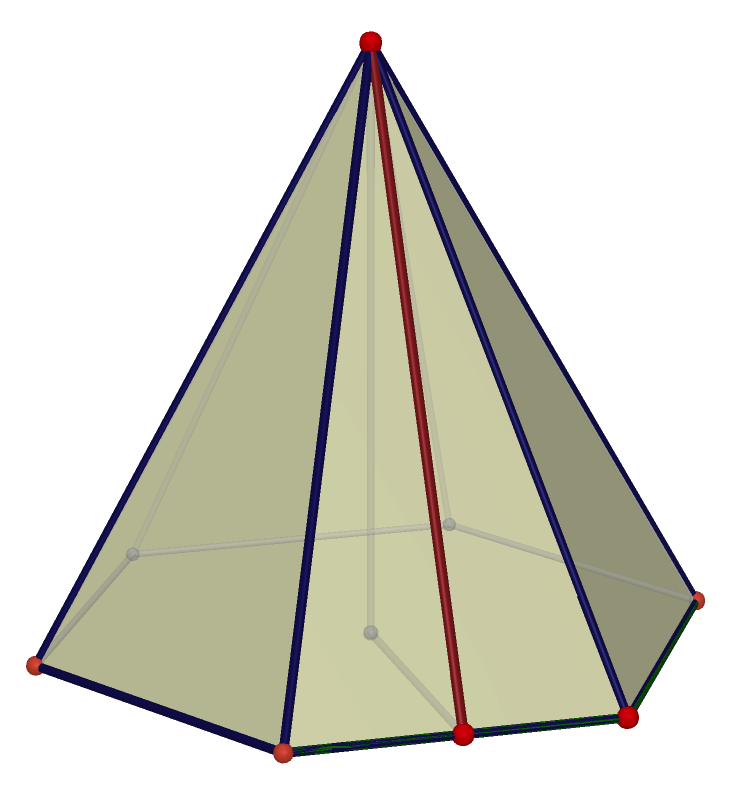
\includegraphics[width=0.25\textwidth]{img-11/piramide6}
\end{center}


\exer  Un triangle rectangle de catets 12 cm i 5 cm gira al voltant d'un dels seus catets generant un con. Calcula l'àrea lateral, l'àrea total i el volum.

\answers{
	Si l'eix de gir és el catet més gran:\par
	Àrea lateral: $65\pi = 204,20$ cm$^2$; àrea total: $90\pi = 282,74$ cm$^2$.
	Volum: $100\pi = 314,159$ cm$^3$.\par
	Si l'eix de gir és el catet menor:\par
	Àrea lateral: $156\pi = 480,09$ cm$^2$; àrea total: $300\pi = 942,48$ cm$^2$.
	Volum $240\pi=753,982$ cm$^3$}

\exer  Tres boles de metall de radis 12 dm, 0,3 m i 4 m es fonen en una sola, Quin serà el diàmetre de l'esfera resultant?

\answers{$D=2\sqrt[3]{65755}=80.72$ dm}

\exer  Quin és la capacitat d'un pou cilíndric d'1,20 m de diàmetre i 20 metres de profunditat?

\answers{$V=\frac{36\pi}{5}=22.619$ m$^3$ o $22\,619$ litres}
 
\exer  Quant cartró necessitarem per construir una piràmide quadrangular regular si volem que el costat de la base mesuri 10 cm i que la seva altura sigui de 25 cm?

\answers{$A_T=100(1+\sqrt{26})=609.91$ cm$^2$}

\exer  Calcula el volum d'un cilindre que té 2 cm de radi de la base i la mateixa altura que un prisma la base del qual és un quadrat de 4 cm de costat i 800 cm${}^{3}$ de volum.

\begin{center}
	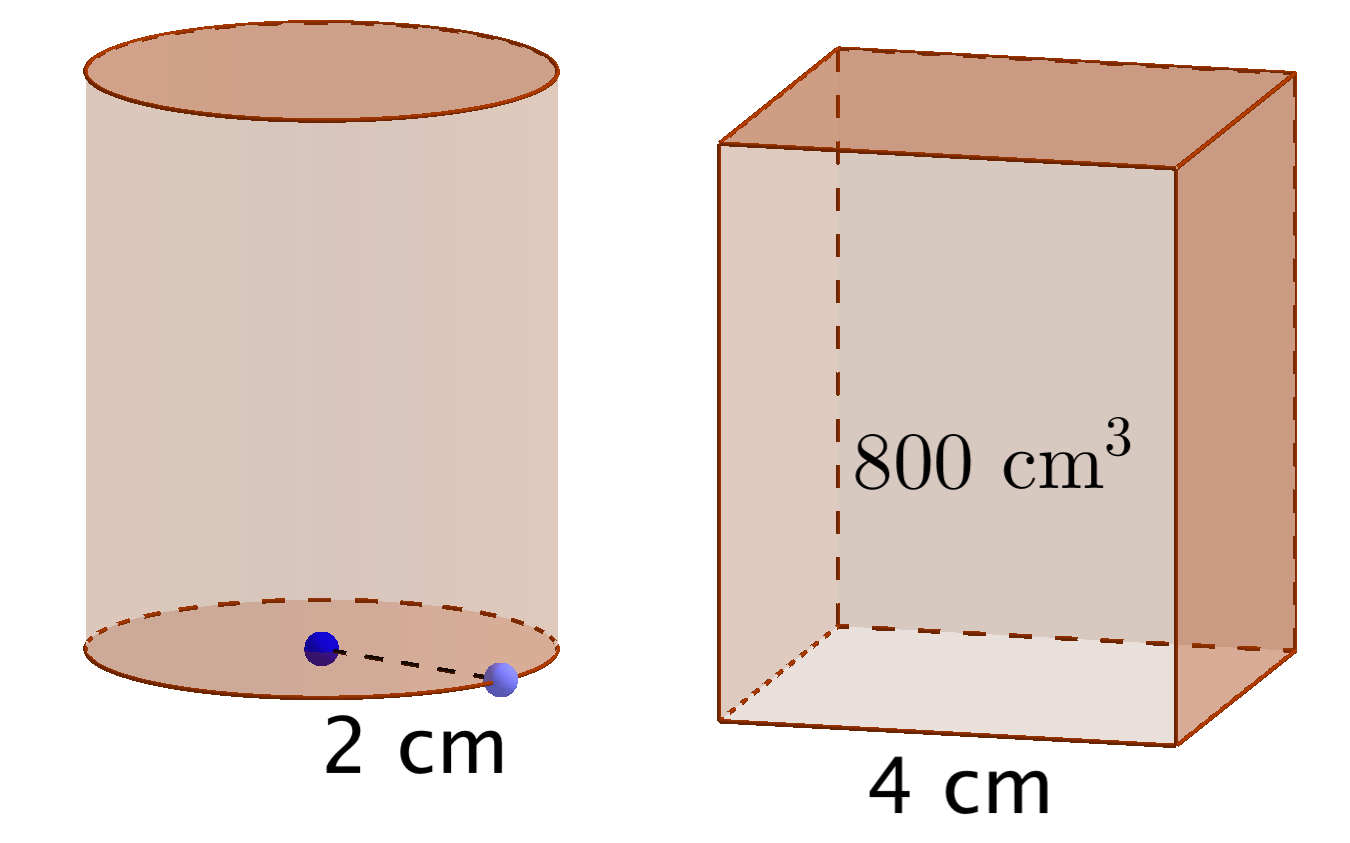
\includegraphics[width=0.4\textwidth]{img-11/pp}
\end{center}

\answers{$V=200\pi=628.319$ cm$^3$}

\exer  Quina és l'àrea de la base d'un cilindre d'1,20 m d'alt i 248 dm${}^{3}$ de volum?

\answers{$A_B=\frac{31}{150}=0.206$ $m^2$ és a dir, té un radi de $R=\sqrt{\frac{0.206}{\pi}}=0.256$ m}

\exer  L'aigua d'una font es condueix fins a uns dipòsits cilíndrics que mesuren 12 m de radi de la base i 20 m d'altura. Després s'embotella en bidons de 2,5 litres. Quants envasos s'omplen amb cada dipòsit? 

\answers{S'omplen $3 619 144$ envasos.}

\exer  Calcula la quantitat de cartolina necessària per construir un anell de 10 tetraedres cadascun dels quals té 2 cm d'aresta. 
\begin{center}
	
\includegraphics[width=0.44\textwidth]{img-11/image655}
\end{center}

\answers{Retallant tots els tetraedres, $A_T=40\sqrt{3}=69.28$ cm$^2$}

\exer En fer el desenvolupament d'un prisma triangular regular de 8 dm d'altura, va resultar un rectangle d'1 metre de diagonal com a superfície lateral. Calcula l'àrea total.

\answers{$A_T=48+2\sqrt{3}=51.46$ cm$^2$}

\exer  Determina la superfície mínima de paper necessària per embolicar un prisma hexagonal regular d'1~m de costat de la base i 2 m d'altura.

\answers{L'àrea total de la figura és $12+3\sqrt{3}=17.194$ m$^2$. Si el volem embolicar amb un rectangle de paper, ha de mesurar 6 m de llarg i 3.74 m d'ample. }


\exer  L'ajuntament ha col·locat unes jardineres de pedra als seus carrers que tenen forma de prisma hexagonal regular. La cavitat interior on es diposita la terra, té 80 cm de profunditat i el costat de l'hexàgon interior és de 60 cm. Calcula el volum de terra que ompliria una jardinera per complet.

\begin{center}
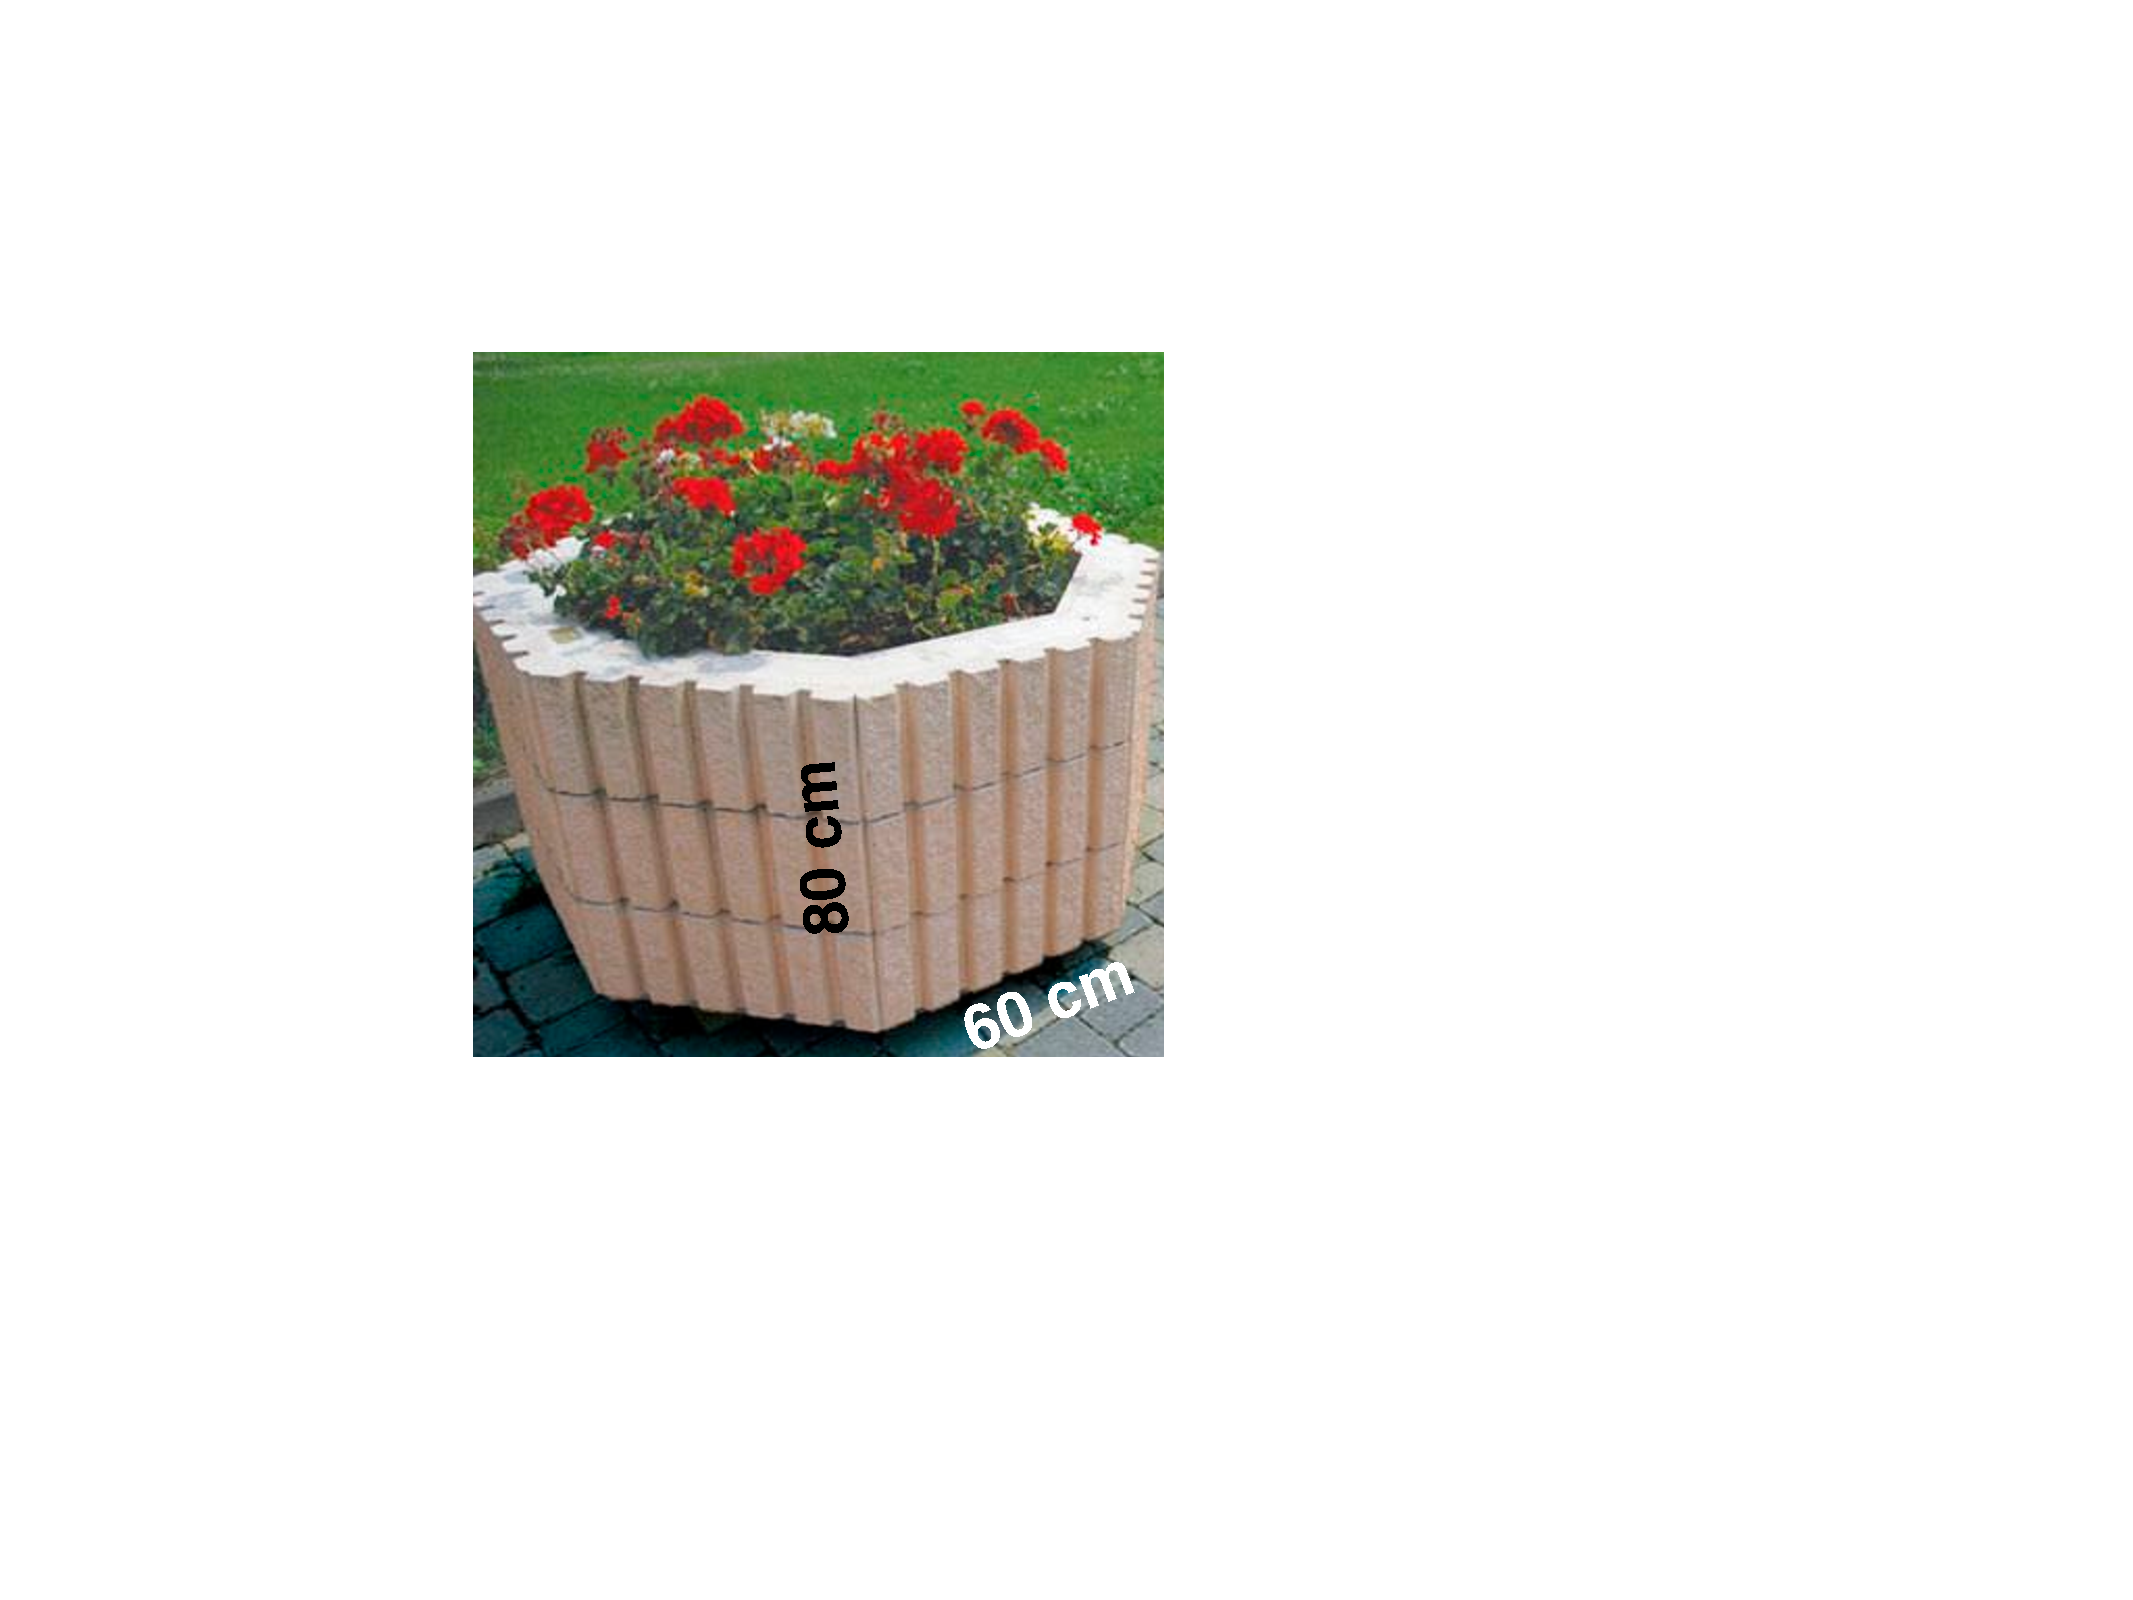
\includegraphics[width=0.3\textwidth]{img-11/jardinera}
\end{center}

\answers{$V=432\sqrt{3}=748.246$ dm$^3$ = litres. L'apotema de la base $a_p=51.96$ cm i l'àrea de la base $A_B=9353.074$ cm$^2$.}

\exer  Una habitació té forma de ortoedre i les seves dimensions són directament proporcionals als nombres 3, 5 i 7. Calcula l'àrea total i el volum si a més se sap que la diagonal mesura 14,5 m.

\answers{Anomenam $r$ a la raó de proporcionalitat. Els costats són $3r$, $5r$ i $7r$. La diagonal és $\sqrt{9r^2+25r^2+49r^2}=14,5$. Obtenim $r=\frac{14,5}{\sqrt{83}}=1.592$. Llavors els costats reals són aproximadament: 4.776, 23.88 i 33.432. \par Amb aquestes dades, l'àrea total $A_T=360$ i el volum $V=423.66$}

\exer  Un ortoedre té 1~dm d'altura i 6~dm${}^{2}$ d'àrea total. La seva longitud és el doble de la seva amplària, quin és el seu volum?

\answers{$V=\frac{21-3\sqrt{33}}{4}=0.942$ dm$^3$}

\exer  Si el volum d'un cilindre de 10 cm d'altura és de 314 cm${}^{3}$, calcula el radi de la base del cilindre. (Utilitza 3,14 com a valor de $\pi$).

\answers{$R=\sqrt{10}=3.2$ cm}
 
\exer  Han instal·lat a casa d'en Joan un dipòsit d'aigua de forma cilíndrica. El diàmetre de la base mesura 2 metres i l'altura és de 3 metres. a) Calcula el volum del dipòsit en m${}^{ 3}$. (Preneu $\pi$=3,14). b) Quants litres d'aigua caben en el dipòsit?

\answers[cols=1]{[$V=3\pi=9.4247$ m$^3$, $9424.8$ litres]}

\exer  Un envàs d'un litre de llet té forma de prisma, la base és un quadrat que té 10 cm de costat. a) Quin és, en cm${}^{3}$, el volum de l'envàs? b) Calcula l'altura de l'envàs en cm.

\answers[cols=1]{[$1$ l = $1000$ cm$^3$, l'altura és 10 cm (és un cub)]}

\exer  Una circumferència de longitud 2,24 cm gira al voltant d'un dels seus diàmetres generant una esfera. Calcula el seu volum. (Preneu$\pi$=3,14).

\answers{Aproximadament 5,885 cm$^3$}

\exer  Una porta fa 2 m d'alt, 80 cm d'ample i 4 cm d'espessor. El preu d'instal·lació és de 200 \euro{} i es cobra 6 \euro{} per m${}^{2}$ en concepte de envernissat, a més del cost de la fusta, que és de 300 \euro{} cada m${}^{ 3}$.

\begin{tasks}
	\task  Calcula el volum de fusta d'una porta. 
	\task  El cost de la fusta d'una porta més la seva instal·lació. 
	\task  El cost del envernissat de cada porta, si només es cobra el envernissat de les dues cares principals. 
\end{tasks}

\answers[cols=1]{[$0.064$ m$^3$, $219.2$ \euro{}, $19.2$ \euro{}]}

\exer  L'aigua continguda en un recipient cònic de 18 cm d'altura i 24 cm de diàmetre de la base s'aboca en un tassó cilíndric de 10 cm de diàmetre. Fins a quina altura arribarà l'aigua?

\answers{$H=34.46$ m}

\exer  Segons Arquimedes quines dimensions té el cilindre circumscrit a una esfera de 5 cm de radi que té la seva mateixa àrea? Calcula aquesta àrea.

\answers{10 cm diàmetre i 10 cm d'altura. L'àrea són $100\pi=314.16$ cm$^2$}

\exer El cristall d'un fanal té forma de tronc de con de 50 cm d'altura i bases de radis 20 i 30 cm. Calcula la seva superfície.
\answers{
	Àrea lateral: $500\pi\sqrt{26} = 8009.52$ cm$^2$.\par
	Si les bases són de vidre, mesuren respectivament $400\pi$ i $900\pi$.  En total serien aproximadament $12093.59$ cm$^2$.}

\exer  Quin és el volum d'una esfera en la qual una circumferència màxima mesura 31,40 m?

\answers{Aproximadament $V=522.803$ cm$^3$}

\exer  Calcula el radi d'una esfera que té 33,51 dm${}^{3}$ de volum.
 
 \answers{$R=2$ dm}
 
\exer  Una piscina mesura 20 m de llarg, 5 m d'ample i 2 m d'alt.

\begin{tasks}
	\task Quants litres d'aigua són necessaris per omplir-la?
	\task Quant costarà recobrir el sòl i les parets amb PVC si el preu és de 20 \euro{}/m${}^{2}$?
\end{tasks}

\answers[cols=1]{[200 m$^3$=200\,000 litres, 4000 \euro{} ]}

\exer[1]  Calcula l'àrea lateral i el volum dels següents cossos geomètrics
\answers[cols=1]{[$A=480$ cm$^2$ i $V=448$ cm$^3$, $A=226.19$ cm$^2$ i $V=282.743$ cm$^3$, $A=$depèn de l'inclinació i $V=125.66$ cm$^3$, $A=277.24$ cm$^2$ i $V=368.61$ cm$^3$]}

\begin{tabular}{cc}	
a) & 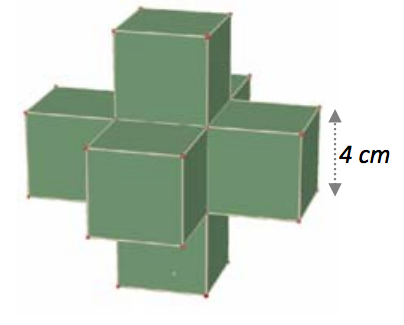
\includegraphics[height=3.5cm]{img-11/87a} \\
\end{tabular}


\begin{tabular}{cc}
b) & 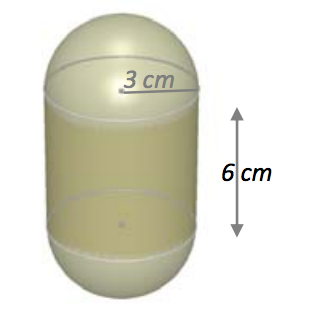
\includegraphics[height=3.5cm]{img-11/87b} \\

c) &  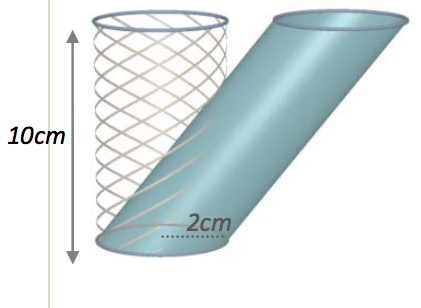
\includegraphics[height=3.2cm]{img-11/87c} \\

d) &  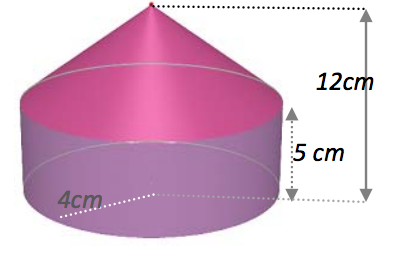
\includegraphics[height=3.2cm]{img-11/87d} \\
\end{tabular}


\exer  En la construcció d'un globus aerostàtic de radi de 2,5 m s'empra lona que té un cost de 300 \euro{}/m${}^{2}$. Calcula l'import de la lona necessària per a la seva construcció.

\answers{Àrea de l'esfera $A=25\pi=78.54$ m$^2$. El cost és 23\,561.95 \euro{}.}

\exer  S'ha pintat per dins i per fora un dipòsit cilíndric sense tapadora de 8 dm d'alt i 3 dm de radi. Tenint en compte que la base només es pot pintar per dins, i que s'ha utilitzat pintura de 2~\euro{}/dm${}^{2}$, quants diners ha costat en total?

\answers{Ha costat 659.73 \euro{}}

\exer  El preu de les teules és de 14,30 \euro{}/m${}^{2}$ Quant costarà re-teular un habitatge la teulada del qual té forma de prisma quadrangular regular de 4 metres d'altura i 8 metres de costat de la base?

\answers{El preu de la piràmide és 1\,294.29 \euro{}}

\exer  S'enrotlla una cartolina rectangular de costats 30 cm i 25 cm de les dues formes possibles, fent coincidir costats oposats. Quin dels dos cilindres resultants té major volum?

\answers{
	Si fem coincidir els costats llargs, el volum és $\frac{9375}{\pi}=2984.15$ cm$^3$. Si fem coincidir
	els costats curts, el volum és $\dfrac{11250}{\pi}=3580.96$ cm$^3$. Aquest darrer és el major.}

\exer  Calcula l'àrea lateral i el volum dels següents cossos geomètrics

\begin{center}
	\scriptsize
	
	\begin{tabular}{p{1cm}p{4cm}}
		
		a) & 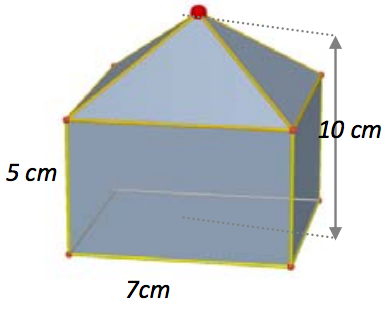
\includegraphics[height=3.5cm]{img-11/88a} \\ & La base és quadrada  \\
		
		b) & 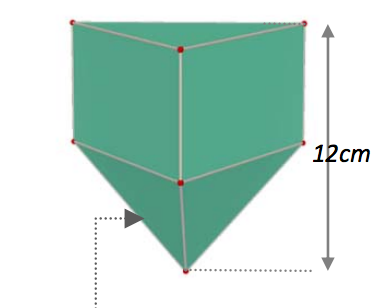
\includegraphics[height=3.5cm]{img-11/88b} \\ &  Tetraedre de 5cm d'aresta \\
	\end{tabular}
\end{center}		
	
\begin{center}
	\scriptsize	
		\begin{tabular}{p{1cm}p{4cm}}	
		
		c) &  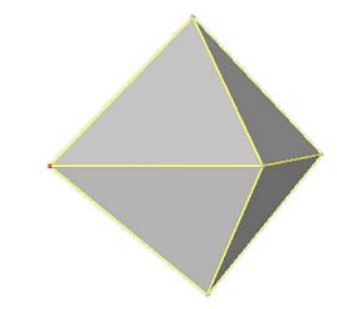
\includegraphics[height=3.2cm]{img-11/88c} \\ & Octàedre de 6cm d'aresta \\
		
		
		d) &  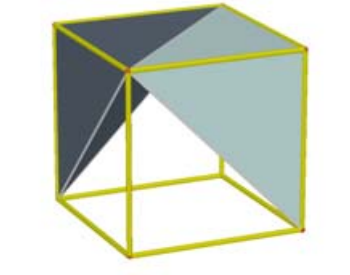
\includegraphics[height=3.2cm]{img-11/88d} \\ & Piràmides construïdes a l'interior d'un cub de 5 dm d'aresta. \\
	\end{tabular}
\end{center}

\answers[cols=1]{[$A=274.45$ cm$^2$; $V=326.6$ cm$^3$,  
				$A=162.06$ cm$^2$; $V=116.64$ cm$^3$, 
				$A=124.71$ cm$^2$; $V=101.82$ cm$^3$, 
				$A=59.15$ dm$^2$; $V=41.6$ dm$^3$]}

\exer  En un recipient cilíndric de 8 dm de diàmetre i que conté aigua, s'introdueix una bola. Quin és el seu volum si després de la immersió puja 0,3 metres el nivell de l'aigua?

\answers{$V=48\pi=150.8$ dm$^3$}

\exer  L'\textit{Atomium} és un monument de Brussel·les que reprodueix una molècula de ferro. Consta de 9 esferes d'acer de 18 m de diàmetre que ocupen els vèrtexs i el centre d'una estructura cúbica de 103 m de diagonal, realitzada amb cilindres de 2 metres de diàmetre. Si utilitzem una escala 1:100 i tant les esferes com els cilindres són massissos, quina quantitat de material necessitarem? 
\begin{center}
	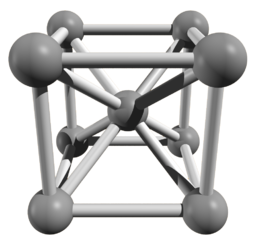
\includegraphics[width=0.25\textwidth]{img-11/atomium}
\end{center}

\answers{En primer lloc hem de calcular el costat del quadrat $x$, per Pitàgores a l'espai $\sqrt{x^2+x^2+x^2}=103$ $\rightarrow$ $x=\frac{103}{\sqrt{3}}=59.47$ m. En segon lloc si l'escala és 1:100 simplement basta reemplaçar la unitat de metres per centímetres. Anem a calcular el volum total de la figura:\par
$V=9 \times \frac{4}{3}\pi 9^3+4\times \pi 1^2 103 + 12 \times \pi 1^2 + 59.47 =9873.64 \pi = 31\,018.95$ cm$^3$ $=0.031$ m$^3$}


\exer \hot Quina de les dues campanes extractores de la figura esquerra té un cost d'acer inoxidable menor?
\vspace{-0.25cm}
\begin{center}
	\hspace{-1cm}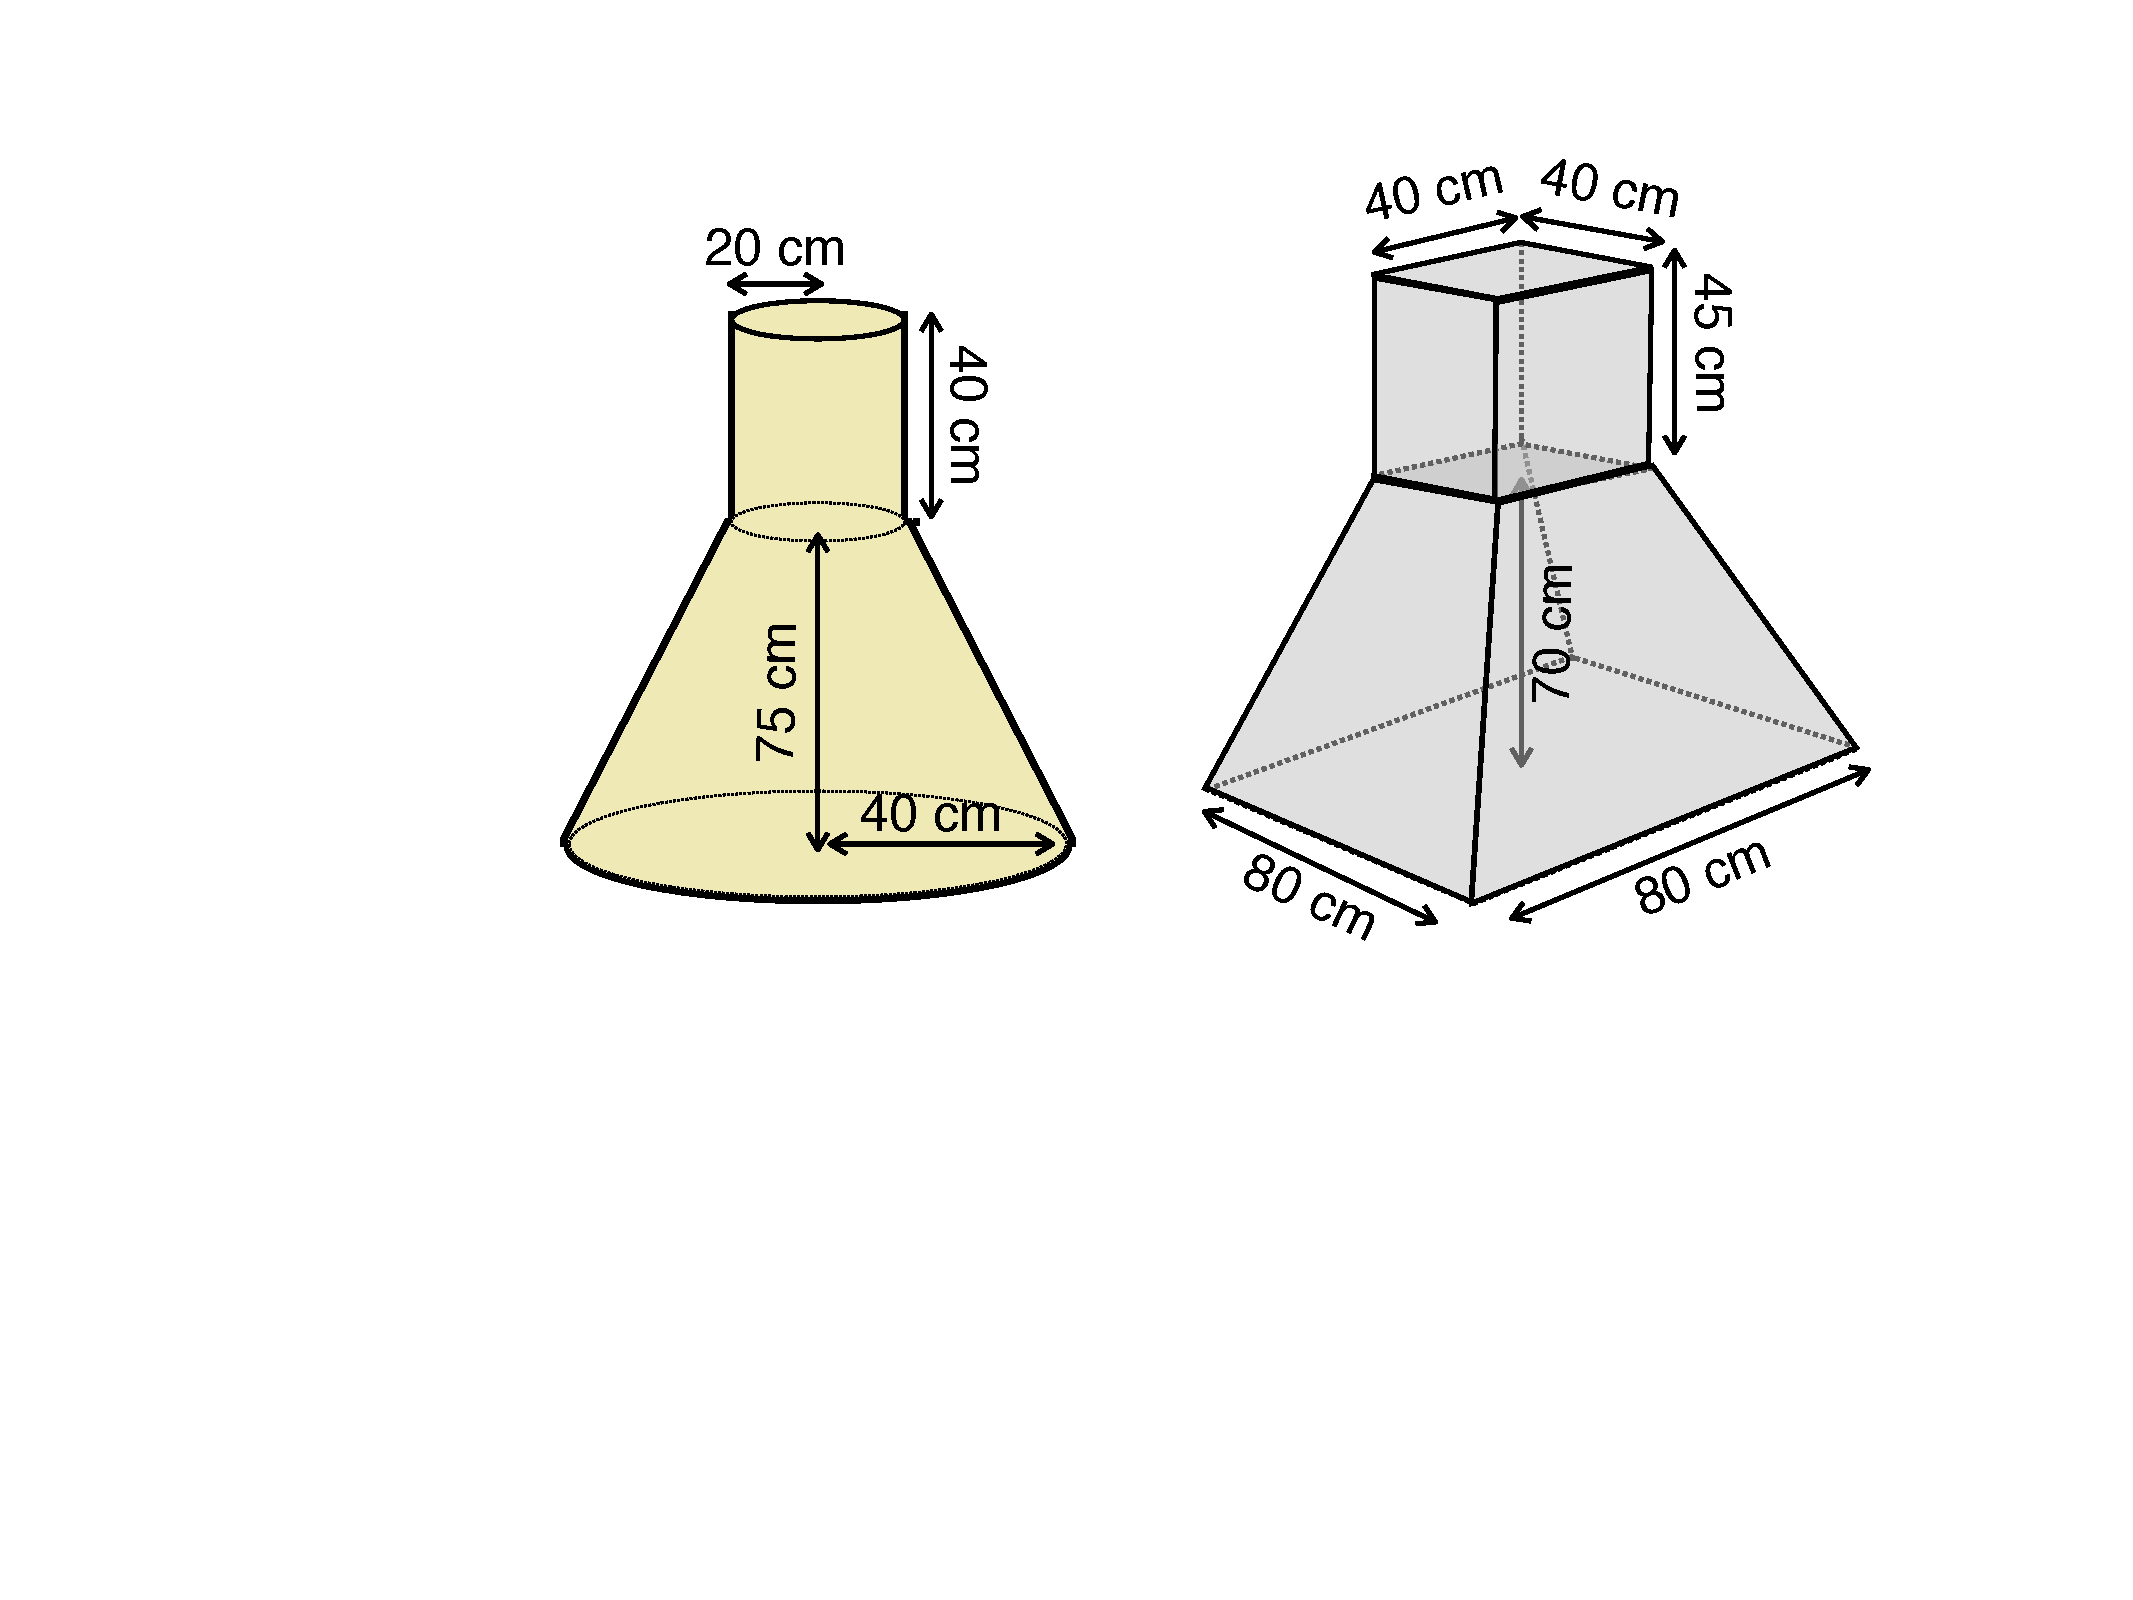
\includegraphics[width=0.45\textwidth]{img-11/campanes}
\end{center}

\answers{La campana circular $A_T=2\pi 20\cdot 40 + \pi \left[ 40\sqrt{40^2+150^2} - 20\sqrt{20^2+75^2} \right]=6257.25\pi=19\,657.74$  cm$^2$ mentre que la campana rectangular $A_T=4\cdot 40\cdot 45 + 4 \cdot \frac{80+40}{2}\cdot 72.801=24\,672.24$. En aquest darrer cas hem hagut de cercar l'altura del trapezi lateral per Pitàgores que ha resultat esser $h=72.801$ cm.\par  L'opció amb menys cost d'acer és la campana circular.}

\exer  Cadascun dels cubs de la figura té 2 cm d'aresta. Quants cal afegir per formar un cub de 216 cm${}^{3}$ de volum? 
\begin{center}
	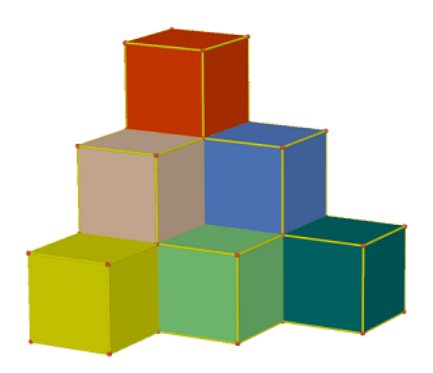
\includegraphics[width=0.3\textwidth]{img-11/cubs}
\end{center}

\answers{17 cubs}

\exer  Un tub d'assaig té forma de cilindre obert en la part superior i rematat per una semiesfera en la inferior. Si el radi de la base és d'1,5 cm i l'altura total és de 15 cm, calcula quants centilitres de líquid caben en ell. 

\answers{$V=\frac{261\pi}{8}=102.49$ cm$^3$= $10.249$ cl}

\exer  Un pot cilíndric de 10 cm de radi i 40 cm d'altura té en el seu interior quatre pilotes de radi 3,5 cm. Calcula l'espai lliure que hi ha en el seu interior.

\begin{center}
\includegraphics[width=0.2\textwidth]{img-11/ous}
\end{center}

\answers{$V=\frac{11314 \pi}{3}=11\,847.993$ cm$^3$}

\exer  La lona d'una ombrel·la oberta té forma de piràmide octogonal regular \linebreak d'1 m d'altura i 45 cm de costat de la base. Es fixa un pal en el sòl en el qual s'encaixa i el vèrtex de la piràmide queda a una distància d'1,80 m del terra. En el moment en què els rajos de sol són verticals, quina superfície d'ombra determina?  
\begin{center}
	\includegraphics[width=0.3\textwidth]{img-11/lona}
\end{center}

\answers{L'ombra és igual al octògon de la base. L'àrea d'un octògon de costat $a$ és
	$A=\frac{2a^2}{\sqrt{3-2\sqrt{2}}}$. Fent que $a=45$ cm, obtenim l'àrea aproximada és de $9\,777.56$ cm$^2$.}

\exer  Construïm un con amb cartolina retallant un sector circular de 120${}^\circ$ i radi 20 cm. Calcula el volum del con resultant.

\answers{$V=\frac{16000\pi}{81}=877.607$ cm$^3$.}

\exer  Un embut cònic de 20 cm de diàmetre ha de tenir 2 litres de capacitat, quina serà la seva altura?

\answers{$H=\frac{60}{\pi}=19,2$ cm}

\exer  En un dipòsit amb forma de cilindre de 25 cm de radi, una aixeta aboca 15 litres d'aigua cada minut. Quant augmentarà l'altura de l'aigua després d'un quart d'hora?

\answers{$H=\frac{360}{\pi}=114.6$ cm}

\exer Una peixera amb forma de prisma recte i base rectangular s'omple amb 56 litres d'aigua. Si té 48 cm de llarg i 36 cm d'ample, quin és la seva profunditat?

\answers{$H=\frac{875}{27}=32.41$ cm}

\exer  Si s'enrotlla una cartolina rectangular de costats 30 cm i 25 cm de les dues formes possibles, quin dels dos cilindres resultants té major volum?

\answers{Veure problema anterior. Aquest està repetit.}

\exer  Un rectangle d'1 m de base i 10 m d'altura gira 360º al voltant d'una recta paral·lela a l'altura, que està situada a 2 m de distància. Calcula la superfície i el volum del cos que resulta.

\answers{$A_T=2 A_B + A_L = 2 \pi (3^2-2^2) + 2\pi 10 (3+2)=110\pi=345.58$ m$^2$ i $V=\pi(3^2-2^2)\cdot 10=157.08$ m$^3$}

\exer  En un gelat de cucurutxo la galeta té 15 cm d'altura i 5 cm diàmetre. Quina és la seva superfície? Si el cucurutxo està completament ple de gelat i sobresurt una semiesfera perfecta, quants grams de gelat conté?

\answers{Superfície de galeta: $\frac{25\pi  \sqrt{37}}{4} =  119,43$ cm$^2$. El volum de gelat és $\frac{125\pi}{4} =  98,175$ cm$^3$. La massa depèn de la densitat del gelat.
 }
 
\end{mylist}

\subsection{Fusos horaris}

 
\begin{mylist}
\exer Quina diferència de longitud existeix entre dues ciutats si la diferència horària entre ambdues és de 5 hores? Podem saber si existeix diferència entre les seves latituds?

\answers{Té $75^\circ$ de longitud. De la latitud no en sabem rés.}

\exer  Un avió emprèn viatge cap a una  ciutat imaginària situada a l'oest de Palma. El viatge dura 10 hores i el seu rumb manté en tot moment la latitud de partida. Si la diferència de longitud entre Palma i la ciutat d'arribada és de 45º i l'avió surt de l'aeroport Son Sant Joan a les 9 del matí. A quina hora local aterrarà a la ciutat de destinació?

\answers{A les 16 hores.}

\exer  La distància entre Londres i Pequín és de 8149 Km i la distància entre Londres i Sao Paulo és de 9508 Km, no obstant això a Pequín el rellotge marca 7 hores més que a Londres i en Sao Paulo 3 hores menys que a Londres. Com expliques aquesta diferència?

\answers{És deu a la diferència de latitud entre els dos llocs.}


\end{mylist}
\end{activitats}

\begin{comment}
\begin{tabular}{|p{1.7in}|p{1.1in}|p{1.1in}|} \hline 
\rowcolor{lightgray}	CIUTAT & LONGITUD & LATITUD \\ \hline 
\cellcolor{lightgray}	LONDRES & 0${}^\circ$ & 51${}^\circ$ 30´ latitud N \\ \hline 
\cellcolor{lightgray}	PEKIN & 116${}^\circ$ longitud E & 40${}^\circ$ latitud N \\ \hline 
\cellcolor{lightgray}	SAO PAULO & 46${}^\circ$ 30´ longitud W & 23${}^\circ$ 30´ latitud S \\ \hline 
\end{tabular}
\end{comment}

\newpage
\begin{autoaval}{55}
\begin{mylist}
	
	\vspace{-2.5cm}
	\exer[2] \begin{minipage}[t]{0.6\textwidth}
		Cadascuna de les rectes r, s, t i p passa per dos vèrtexs consecutius d'un octàedre tal com s'observa en la figura. Assenyala quina afirmació de les següents és vertadera:
		
		
		\begin{tasks}
			\task  Les rectes r i s són coplanàries i secants.
			\task  Les rectes t i p no són coplanàries.
			\task  Les rectes r i p es creuen.
			\task  r i s contenen arestes d'una mateixa cara de l'octàedre 
		\end{tasks}
	
	\end{minipage}
	\begin{minipage}{0.4\textwidth}
		\centering
		\vspace{2.5cm}
		\includegraphics[width=0.7\textwidth]{img-11/octaedrerectes}
	\end{minipage}
	
 	\answers{\textbf{--9.} Autoavaluació: 1c; 2a; 3d; 4b; 5a; 6d; 7b; 8a; 9c.}



\exer  Observa els següents cossos geomètrics i selecciona l'opció vertadera:
	\hspace{-0.25cm}
\begin{center}
	\begin{tabular}{cccccc}
		I) & II) & III) & IV) & V) & VI) \\
      \includegraphics[height=2cm]{img-11/image672} &
 \includegraphics[height=1.5cm]{img-11/image673} &
  \includegraphics[height=1.5cm]{img-11/image674} &
   \includegraphics[height=1.5cm]{img-11/image675} &
    \includegraphics[height=1.5cm]{img-11/image676} &
     \includegraphics[height=1.5cm]{img-11/image677}
    \end{tabular}
 \end{center}
 
     \begin{tasks}(2)
	\task*  Els cossos I), II), IV) i V) compleixen la relació de Euler.
	\task*  Hi ha dos cossos de revolució III) i VI).
	\task  Són poliedres regulars II) i IV).
	\task  Són còncaus I) i V).
\end{tasks}


\exer  Si l'altura d'un prisma de base quadrada és 10 cm i el costat de la base és 4 cm, la seva àrea total és:

\begin{tasks}(4)
	\task  160 cm${}^{2}$    
	\task  320 cm${}^{2}$   
	\task  400 cm${}^{2}$   
	\task  192 cm${}^{2}$
\end{tasks}


\exer  Un dipòsit d'aigua té forma de prisma hexagonal regular de 5 m d'altura i costat de la base 1 m. Si només conté les tres quartes parts de la seva capacitat, el nombre aproximat de litres d'aigua que hi ha en ell és:

\begin{tasks}(4)
	\task  13000 l    
	\task  9750 l   
	\task  3750 l 
	\task  3520 l
\end{tasks}


\exer  La teulada d'una caseta té forma de piràmide quadrangular regular d'1,5 m d'altura i 80 cm de costat de la base. Si es necessiten 15 teules per metre quadrat per recobrir la teulada, en total s'utilitzaran: 

\begin{tasks}(4)
	\task  38 teules   
	\task  76 teules   
	\task  72 teules 
	\task  36 teules
\end{tasks}

	\exer  Una caixa de dimensions 30~x~20~x~15~cm, està plena de cubs d'1 cm d'aresta. Si s'utilitzen tots per construir un prisma recte de base quadrada de 10 cm de costat, l'altura mesurarà:

\begin{tasks}(4)
	\task  55 cm    
	\task  65 cm   
	\task  75 cm   
	\task  90 cm
\end{tasks}


\end{mylist}
\end{autoaval}
\newpage

\begin{autoaval}{15}
	\setcounter{myenumi}{6}
	\begin{mylist}
		
	
\exer  El radi d'una esfera que té el mateix volum que un con de 5 dm de radi de la base i 120 cm d'altura és:

\begin{tasks}(4)
	\task  $5\sqrt{3} $ dm  
	\task  $\sqrt[{3}]{75} $ dm   
	\task  150 cm   
	\task  $\sqrt[{3}]{2250} $ cm
\end{tasks}


\exer  Es distribueixen 42,39 litres de dissolvent en llaunes cilíndriques de 15 cm d'altura i 3 cm de radi de la base. El nombre d'envasos necessari és: 

\begin{tasks}(4)
	\task  100    
	\task  10    
	\task  42    
	\task  45
\end{tasks}


\exer  L'àrea lateral d'un tronc de con que té 20 cm d'altura i bases de radis 30 i 15 cm, és:

\begin{tasks}(4)
	\task  2250 $\pi$ cm${}^{2}$   
	\task  900 $\pi$ cm${}^{2}$   
	\task  1125 $\pi$ cm${}^{2}$   
	\task  450 $\pi$ cm${}^{2}$ 
\end{tasks}

\begin{comment}

\exer  De les coordenades geogràfiques de les ciutats A, B, C  quina afirmació és correcta


\begin{longtable}{|p{1.1in}|p{1.1in}|p{1.1in}|} \hline 
\rowcolor{lightgray} CIUTAT & LONGITUD & LATITUD \\ \hline 
A & 15${}^\circ$ E & 15${}^\circ$ N \\ \hline 
B & 15${}^{o }$W & 15${}^\circ$ N \\ \hline 
C & 15${}^\circ$ E & 15${}^\circ$ S \\ \hline 
\end{longtable}
\begin{tasks}
\task  Les ciutats A i B tenen la mateixa hora i la ciutat C dues hores menys.
\task  Les ciutats A i B tenen la mateixa hora i la ciutat C dues hores més.
\task  Les ciutats A i C tenen la mateixa hora i la ciutat B dues hores més.
\task  Les ciutats A i C tenen la mateixa hora i la ciutat B dues hores menys.
\end{tasks}

\end{comment}

\end{mylist}
\end{autoaval}

\vspace{2cm}

 \resum
\label{sec:resum11}

\begin{center}
	\renewcommand{\arraystretch}{1.3}
\begin{longtable}{|p{0.6\textwidth}|p{0.35\textwidth}|} \hline 
	
   \rowcolor{lightgray}\multicolumn{2}{|p{\textwidth}|}{\textbf{Poliedre. Elements d'un poliedre.  Tipus de poliedres}} \\ \hline 
   
   Un poliedre és una regió tancada de l'espai limitada per polígons. Els seus principals elements són: cares, arestes, vèrtexs, angles diedres i poliedres, així com les diagonals.\newline Els poliedres poden ser còncaus i convexos depenent que alguna de les seves cares sigui un polígon còncau o cap ho sigui.\newline Entre els poliedres destaquen poliedres regulars, prismes i piràmides. & 
\begin{center}
\includegraphics[height=2cm]{img-11/cubs}
\includegraphics[height=2cm]{img-11/piramide6}

\includegraphics[height=2cm]{img-11/dodecaedre}
\includegraphics[height=2cm]{img-11/prisma-hexagonal}
\end{center}
\\ \hline 

  \rowcolor{lightgray}\multicolumn{2}{|p{\textwidth}|}{\textbf{Teorema d'Euler}} \\ \hline 


 En tot poliedre convex el nombre de cares més el nombre de vèrtexs és igual al nombre d'arestes més 2. & \[C + V = A + 2\] \\ \hline
 
   \rowcolor{lightgray}\multicolumn{2}{|p{\textwidth}|}{\textbf{Poliedres regulars}} \\ \hline 
  
 Un poliedre regular és un poliedre que compleix que totes les seves cares són polígons regulars iguals i que els seus angles poliedres són iguals.\newline  Hi ha cinc poliedres regulars: tetraedre (4 cares), cub (6 cares), octàedre (8 cares), dodecaedre (12 cares) i  icosàedre (21 cares) & 
 \begin{center}
 	\includegraphics[height=1.5cm]{img-11/tetraedro}
 	\includegraphics[height=1.5cm]{img-11/poliedro-convexo}
 	\includegraphics[height=1.5cm]{img-11/octaedre}
 	
 	\includegraphics[height=2cm]{img-11/dodecaedre}
 	\includegraphics[height=2cm]{img-11/icosaedre}
 \end{center}
 
  \\ \hline 
 
   \rowcolor{lightgray}\multicolumn{2}{|p{\textwidth}|}{\textbf{Prismes}} \\ \hline 
  
   Un prisma és un poliedre determinat per dues cares paral·leles que són polígons iguals i tantes cares laterals com a costats tenen les bases.\newline Poden ser còncaus o convexos; rectes o oblics, regulars o irregulars; triangulars, quadrangulars, pentagonals{\dots}\  &
   
    \begin{center}
   	\includegraphics[height=2.2cm]{img-11/prisma-hexagonal}
   	\includegraphics[height=2.2cm]{img-11/desenvolupa2}
   \end{center}
   
 \\ \hline 
   
     \rowcolor{lightgray}\multicolumn{2}{|p{\textwidth}|}{\textbf{Teorema de Pitàgores a l'espai}} \\ \hline 
   
   
  La diagonal d'un ortoedre és l'arrel quadrada de la suma dels quadrats de les seves arestes 
  \[D^2 = a^2 + b^2 + c^2 \]
   & 
    \begin{center}
   	\includegraphics[height=3cm]{img-11/pitagores-espai}
   \end{center}
    \\ \hline 
    

    \rowcolor{lightgray}\multicolumn{2}{|p{\textwidth}|}{\textbf{Piràmides}} \\ \hline 
  
  
Una piràmide és un poliedre determinat per una cara poligonal denominada base i tantes cares triangulars amb un vèrtex comú, com a costats té la base.\newline Poden ser còncaves o convexes; rectes o obliqües, regulars o irregulars; triangulars, quadrangulars, pentagonals{\dots} & 
  \begin{center}
	\includegraphics[height=2.5cm]{img-11/piramide6}
\end{center}
\vspace{-1cm}
 \\ \hline 

  \rowcolor{lightgray}\multicolumn{2}{|p{\textwidth}|}{\textbf{Tronc de piràmide}} \\ \hline 

  Un tronc de piràmide és el poliedre resultant en tallar una piràmide per un pla paral·lel a la base. Les bases són polígons semblants i les cares laterals són trapezis. & 
    \begin{center}
  	\includegraphics[height=2cm]{img-11/tronc11}
  \end{center}\vspace{-1cm}
    \\ \hline 
  
    \rowcolor{lightgray}\multicolumn{2}{|p{\textwidth}|}{\textbf{Cossos de revolució}} \\ \hline 
  
 Els cossos de revolució són cossos geomètrics que s'obtenen en fer girar una línia al voltant d'una recta fixa denominada \textit{eix}. La línia que gira es diu \textit{generatriu}.\newline Entre els cossos de revolució destaquen cilindres, cons i esferes. &  
  \begin{center}
 	\includegraphics[height=2cm]{img-11/cilindro}
 	\includegraphics[height=2cm]{img-11/cono}
 	\includegraphics[height=2cm]{img-11/esfera}
 \end{center}\vspace{-1cm}
  \\ \hline 
  \newpage
   \rowcolor{lightgray}\multicolumn{2}{|p{\textwidth}|}{\textbf{Àrees lateral i total d'un prisma}} \\ \hline 
 
 
  \[A_{Lateral} =\textbf{Perímetre}_{Base} \; \cdot \; Altura\]  \[A_{total} =\quad\text{Àrea}_{Lateral} \; +\; 2 \text{Àrea}_{Base} \] & \begin{center} \includegraphics[height=2.3cm]{img-11/despliegue1} \end{center} \vspace{-0.5cm}\\ \hline 
  
  \rowcolor{lightgray}\multicolumn{2}{|p{\textwidth}|}{\textbf{Àrees lateral i total d'una piràmide regular}} \\ \hline 
  
  
  \[ A_{Lateral} =\frac{\textbf{Perímetre}_{Base} \; .\; Apotema_{\textbf{piràmide}} }{2}\]   \[A_{total} =\quad \text{Àrea}_{Lateral} \; +\; \text{Àrea}_{Base} \] & \begin{center} \includegraphics[height=2.5cm]{img-11/despliegue2} \end{center} \vspace{-0.5cm}\\ \hline 


   \rowcolor{lightgray}\multicolumn{2}{|p{\textwidth}|}{\textbf{Àrees lateral i total d'un tronc de piràmide regular}} \\ \hline 


 \[ A_{Lateral} =\frac{\textbf{Perímetre}_{Base} \; .\; Apotema_{tronc} }{2}\]   \[A_{total} =\quad \text{Àrea}_{Lateral} \; +\; \text{Àrea}_{Base\; 1} +\; \text{Àrea}_{Base\; 2} \] & \begin{center} \includegraphics[height=2cm]{img-11/tronc11}  \includegraphics[height=2.5cm]{img-11/desenvolupa6} \end{center}\vspace{-0.5cm} \\ \hline 
 

  \rowcolor{lightgray}\multicolumn{2}{|p{\textwidth}|}{\textbf{Àrees lateral i total d'un cilindre}} \\ \hline 
 
 
  \[A_{Lateral} =\quad 2\; \pi \; R\; H\] \[A_{total} =\quad 2\; \pi \; R\; H\; \; +\; \; 2\; \pi \; R^{2} \] & \begin{center} \includegraphics[height=2cm]{img-11/cilindro} \includegraphics[height=2cm]{img-11/desenvolupa5}  \end{center}\vspace{-0.5cm} \\ \hline 
  
    \rowcolor{lightgray}\multicolumn{2}{|p{\textwidth}|}{\textbf{Àrees lateral i total d'un con}} \\ \hline 
  
\[A_{Lateral} =\quad \pi \; R\; G\] \[A_{total} =\quad \pi \; R\; G+\; \pi \; R^{2}\] & \begin{center} \includegraphics[height=2cm]{img-11/cono} \includegraphics[height=2cm]{img-11/desenvolupa7} \end{center} \\ \hline 

  \rowcolor{lightgray}\multicolumn{2}{|p{\textwidth}|}{\textbf{Àrees lateral i total d'un tronc de con}} \\ \hline 

\[A_{Lateral} =\quad \left(\pi \; R+\pi \; r\right)\; G\] \[A_{Total}= A_{Lateral} + \pi R^2 + \pi r^2 \] & \begin{center} \includegraphics[height=2cm]{img-11/desenvolupa3} \end{center}\vspace{-0.5cm} \\ \hline 



  \rowcolor{lightgray}\multicolumn{2}{|p{\textwidth}|}{\textbf{Àrea i volum d'una esfera}} \label{sec:resumvolums} \\ \hline 

  \[ A_{total} =\quad 4\; \pi \; R^{2}\] \[Volum=\quad \frac{4}{3} \pi \; R^{3}\] & \begin{center} \includegraphics[height=2cm]{img-11/esfera} \end{center}\vspace{-0.5cm}\\ \hline

  \rowcolor{lightgray}\multicolumn{2}{|p{\textwidth}|}{\textbf{Volum d'un prisma i d'un cilindre}} \\ \hline 
   
 \[Volum=\quad \text{Àrea}_{base} \; \cdot\; Altura\] & \begin{center} \includegraphics[height=2cm]{img-11/ortoedre} \includegraphics[height=2cm]{img-11/cilindro} \end{center}\vspace{-0.5cm} \\ \hline 


  \rowcolor{lightgray}\multicolumn{2}{|p{\textwidth}|}{\textbf{Volum d'una piràmide i d'un con}} \\ \hline 
  
 \[Volum=\quad \frac{\text{Àrea}_{base} \; \cdot \; Altura}{3} \] &  \begin{center} \includegraphics[height=2cm]{img-11/piramide6} \includegraphics[height=2cm]{img-11/cono} \end{center} \vspace{-0.5cm} \\ \hline 

  
  \rowcolor{lightgray}\multicolumn{2}{|p{\textwidth}|}{\textbf{Coordenades geogràfiques}} \\ \hline 
  
  
 \textbf{Latitud}: Distància del punt geogràfic a l'Equador mesurada sobre el meridià que passa pel punt.\newline \textbf{Longitud:} Distància del punt geogràfic al meridià zero o de Greenwich, mesurada sobre el paral·lel que passa pel punt. & \begin{center} \includegraphics[height=2.2cm]{img-11/coordenadas} \end{center}  \vspace{-0.5cm}\\ \hline 

  \rowcolor{lightgray}\multicolumn{2}{|p{\textwidth}|}{\textbf{Fusos horaris}} \\ \hline 

 Cada \textbf{fus horari} és una zona del globus terraqüi compresa entre dos meridians que es diferencien en 15${}^{\circ}$ de longitud.  & \begin{center} \includegraphics[height=2.2cm]{img-11/planisferi} \end{center}\vspace{-0.5cm}  \\ \hline 
\end{longtable}
\end{center}
 
